\chapter{Numerical Methods}\label{chap:2}
In this chapter, we will discuss the fundamentals of \textcolor{red}{the} numerical methods \textcolor{red}{for} solving the Navier-Stokes equations.
We begin the discussion of the method weighted of residuals (\S \ref{sec:methodofweightedresiduals}) and the spatial discretisation using spectral/\emph{hp} element methods in one dimension (\S \ref{sec:spectralhpelementmethods}).
This is followed by techniques for solving the Navier-Stokes equations (\S \ref{sec:numeraltechniquesforNS}), such as the velocity-correction scheme, enforcing a constant flow rate and the quasi-3D approach for semi-homogeneous domains. 
This chapter concludes with \textcolor{red}{introducing the} numerical techniques for performing stability analysis of the Navier-Stokes equations (\S \ref{sec:stabilityanalysisofNS}), including eigenvalue computation and edge tracking.
% In this chapter, I will present the numerical methods ultilised in this thesis.
% The premise of numerical methods is to solve for the the partial differential equations, the Navier-Stokes equations.
% The incompressible Navier-Stokes equations describe the time- and spatial-varying velocity field and pressure field.
% One of the foundations of solving partial differential equations begin with the method of weighted residuals. 

%%%%%%%%%%%%%%%%%%%%%%%%%%%%%%%%%%
% 3.1 METHOD OF WEIGHTED RESIDUALS
%%%%%%%%%%%%%%%%%%%%%%%%%%%%%%%%%%

\section{Method of weighted residuals}\label{sec:methodofweightedresiduals}
Spatial discretisation errors, or residuals, arise as one seeks an approximate solution to \textcolor{red}{a partial} differential equation (PDE).
The method of weighted residuals provides a generic mathematical framework in which constraints on the residual could be applied flexibly, defining the spatial discretisation scheme and its convergence properties.
We approximate the solution of PDE by considering a finite expansion of a suitable basis, to which its coefficients are sought after by minimising the inner product between the PDE and a test (or weight) function.
To demonstrate this, we consider a linear partial differential equation as,
\begin{equation}\label{eq:linear_operator}
    \mathbf{L}[u(x)] = 0, \quad x \in \Omega,
\end{equation}
where $\mathbf{L}$ refers to a linear spatial differential operator subjected to some boundary conditions within the domain, $\Omega$, while $u(x)$ refers to the exact solution of $\mathbf{L}$.
Examples of PDEs with linear spatial differential operators include the Laplace equation, $\nabla^2 u = 0 $, Poisson equation, $\nabla^2 u - f = 0$, and the Helmholtz equation, $\nabla^2 u - \lambda u  + f = 0$.
We \textcolor{red}{assume} that the exact solution $u(x)$ can be approximated (discretised) by $N$ finite number of global basis (or expansion) functions, $\Phi_i(x)$.
\begin{equation}\label{eq:approximate}
    u(x) \approx u^\delta(x) = \sum_{i=0}^{N-1} \hat{u}_i \Phi_i(x),
\end{equation}
where $u^\delta(x)$ refers to the approximate solution of $u(x)$, consisting of a linear combination of the product between the $i^{th}$ basis coefficient, $\hat{u}_i$, and the $i^{th}$ global basis expansion, $\Phi_i(x)$, defined within $\Omega$.
Since $u^\delta(x)$ is an approximate solution of equation \eqref{eq:helmholtz}, we expect a residual (or error) between the exact solution, $u(x)$, and $u^\delta(x)$,
\begin{equation}\label{eq:residual}
    \mathbf{L}[u^\delta(x)] = R[u^\delta(x)],
\end{equation}
where $R[u^\delta(x)]$ refers to the residual which depends on the approximate solution $u^\delta(x)$ and varies within $\Omega$.
In other words, equation \eqref{eq:residual} might not be satisfied everywhere in $\Omega$. 
Next, we need to place restrictions on the residual, such that it the residual approaches zero, $R \rightarrow 0$, and the approximate solution approaches the exact solution, $u^\delta(x) \rightarrow u(x)$.
The method of weighted residuals places a restriction on the residual by applying an inner product between the governing equation, and $N$ test (or weight) functions, $v_j(x)$, and setting it to zero,
\begin{equation}\label{eq:weightinnerresidual}
    (v_j(x), R[u^\delta(x)]) = 0, \quad j = 0, ..., N-1.
\end{equation}
\begin{definition}[Inner product]
The inner product between two functions $f(x)$ and $g(x)$ is,
\begin{equation}
       (f, g) = \int_\Omega f(x) g(x) dx \nonumber.
\end{equation}
\end{definition}
% where $(\, \cdot \, , \, \cdot \,)$ refers to an inner product, a measure of orthogonality between function $f(x)$ and $g(x)$ defined as,
% \begin{equation}\label{eq:inner-product}
%        (f, g) = \int_\Omega f(x) g(x) dx.
% \end{equation}
By enforcing equation \eqref{eq:weightinnerresidual}, the discrete problem becomes a system of $N$ ordinary differential equations to solve for the $N$ basis coefficients, $\hat{u}_i$.
The choice of test function defines the projection methods, and examples of different projection methods are shown in table \ref{tab:weightFunction}.
We emphasise that the method of weighted residuals only describes the projection method, but does not specify the type of basis expansions, as we will discuss later in \S \ref{sec:spectralhpelementmethods}.
The choice of projection method coupled with suitable basis expansions will have different solution convergence properties.
Of particular interest is on how quickly the residual vanishes as the number of basis expansions increases.
For instance, by considering the Galerkin method coupled with Fourier expansions, one can expect exponential convergence for a sufficiently smooth problem which is desirable for an efficient representation of turbulent dynamics.
% Certain mathematical properties such as spectral convergence as desired in the case of Galerkin projection using Fourier expansions, 
% The choice of \emph{trial} functions used in \emph{nektar++} will be elaborated in Section \ref{sec:modifiedBasis}.
% the method of weighted residuals is only restrictive to the weight
% Table \ref{tab:weightFunction} shows the different forms of weight functions and its corresponding numerical method.
\renewcommand{\arraystretch}{1.5} % Default value: 1
\begin{table}[h]
    \centering
        \begin{tabular}{cc}
            Weight functions & Projection method \\
            \hline
            $v_j(x) = \delta(x-x_j)$ & Collocation \\
            $v_j(x) =\left\{\begin{array}{ll}
                1 & \mbox{if } x \in \Omega_j\\
                0 & \mbox{if } x \notin \Omega_j \\
           \end{array}\right. $& Finite-Volume \\
            $v_j(x) = \phi_j$& Galerkin \\
            $v_j(x) = \frac{\partial R}{\partial \hat{u}_j}$ & Least-squares \\
            \hline
        \end{tabular}
        \caption{Examples of weight functions and projection methods}
    \label{tab:weightFunction}
\end{table}
% For instance, for $v_j = \delta(x-x_j)$, the numerical method becomes the \emph{collocation} method where the differential equation is satisfied on discrete points $x_j$.
% The type of restriction on the residual is implemented through the choice of \emph{test} function, $v_j$.
\section{Galerkin Projection}\label{sec:galerkinprojection}
Galerkin projection remains as a standard projection method in the context of the finite element methods, where the test functions, $v(x)$, are chosen to be lie in the same functional space as the global basis functions, $\Phi(x)$.
To demostrate the Galerkin projection method, we consider that the differential operator earlier in equation \eqref{eq:linear_operator} as a 1D Helmholtz equation,
\begin{subequations}\label{eq:helmholtz}
    \begin{equation}
        \mathbf{L}[u(x)] \equiv \frac{\partial^2 u(x)}{\partial x^2} - \lambda u(x) + f(x) = 0, \quad x \in \Omega := [0, l]
    \end{equation}
    \begin{equation}
        u(0) = g_D, \quad \frac{\partial u}{\partial x}\Big|_{x=l} = g_{N}.
    \end{equation}
\end{subequations}
where $\lambda$ is a real positive constant, $f(x)$ is a forcing function, and $\Omega$ refers to the spatial domain bounded between $0$ and $l$. 
% $ hh u(x), \lambda, f, \Omega$ refers to the linear (spatial) differential operator, solution to the diffential equation, a real positive constant, forcing function and the spatial domain bounded between 0 and $l$, respectively.
To ensure that problem is well posed, Dirichlet and Neumann boundary conditions, $g_D$ and $g_N$, are imposed at $x = 0$ and $x = l$ respectively.
% In order for the problem to be well-posed, we impose both Dirichlet and Neumann, boundary conditions corresponding to $g_D$ and $g_N$ at $x= 0 $ and $x=l$, respectively.
Equation \ref{eq:helmholtz} is commonly referred to as the strong or classical form.

The subsequent step is to take the inner product of the equation \eqref{eq:helmholtz} with a test function, $v(x)$, that satisfies the homogeneous Dirichlet boundary conditions by definition, i.e. $v(0) = 0$, and setting the inner product to zero,
\begin{equation}\label{eq:helmholtz_inner}
    (v(x), \, \mathbf{L}[u(x)]) = \int_0^l v(x) \left[\frac{\partial^2 u(x)}{\partial x^2} - \lambda u(x) + f(x)\right] \mathrm{d}x =  0,
\end{equation}
akin to applying the method of weighted residuals (\S \ref{sec:methodofweightedresiduals}). Next, we perform integration by parts,
\begin{subequations}
    \begin{equation}\label{eq:weak_form}
        \underbrace{\int_0^l \frac{\partial v}{\partial x}\frac{\partial u}{\partial x} \, \mathrm{d}x + \int_0^l \lambda v u \, \mathrm{d}x}_{a(v,u)}= \underbrace{\int_0^l v f \, \mathrm{d}x + \left[ v \frac{\partial u}{\partial x} \right]_0^l}_{f(v)}.
    \end{equation}
    \begin{equation}\label{eq:compact}
        a(v,u) = f(v).
    \end{equation}
\end{subequations}
Equation \eqref{eq:weak_form} is typically referred to as the weak \footnote{The notions of the \emph{weak} and \emph{strong} forms refer to the smoothness (regularity) required of admissible solutions. In the weak formulation, the highest derivative involved is up to first-order, so the solution space is $H^1$. This space is generally larger than that of the strong formulation, which required $u \in \mathcal{H}^2(\Omega)$. Since $H^2(\Omega) \subset H^1(\Omega)$ the weak formulation imposesd a `less stringent' constraint of the solution space of admissible functions.} form of equation \eqref{eq:helmholtz}.
The weak form can be represented in compact notation in equation \eqref{eq:compact}, where $a(v,u)$ is bilinear and symmetric. In structural mechanics, $a(u,u)$ is commonly referred to as the \textit{strain} energy.
To ensure that the \textit{strain} energy is finite, we restrict the choice of solutions $u(x)$ to lie in the solution space,
\begin{equation}\label{eq:solution_space}
    \mathcal{U} := \{ u \, | \, u \in H^1(\Omega), u(0) = g_D \},
\end{equation}
% where $u \in H^1$ contains functions of $u$ in the Sobolev space such that the Dirichlet condition $u(0) = g_D$ is statisfied and the sum of square integral of $u$ and its first derivatives, $\frac{\partial u}{\partial x}$ remains bounded,
where $u \in H^1$ refers to functions of $u$ belonging to Sobolev space of order 1, and satistfying the Dirichlet condition, $u(0) = g_D$,  at $x = 0$.
\begin{definition}[Sobolev space]
    We define Sobolev space of order $n \geq 1$ on $\Omega$,
    \begin{equation}
        H^n(\Omega) = \{u \, | \, u \in L_2(\Omega), D^\alpha u \in L_2(\Omega), \forall \alpha : \alpha \leq n\}, \nonumber
    \end{equation}
    where $D^\alpha u$ refers to derivatives up to order $\alpha$ and $L_2(\Omega)$ refers to functions that are square integrable.
\end{definition}
\begin{definition}[$L_2$ space]
    The space $L_2(\Omega)$ refers to functions that are square integrable,
    \begin{equation}
        (u, u)_{L_2} = \int_\Omega |u(x)|^2 \, \mathrm{d}\Omega < \infty. 
    \end{equation}
\end{definition}
In other words, $H^1$ functions satisfy the condition that the integral of the square of the function and its first derivative is finite, consistent with the highest order derivative in the weak formulation of equation \eqref{eq:helmholtz_inner}.
Similarly, the space of test functions, $\mathcal{V}$, is defined as,
\begin{equation}\label{eq:test_space}
    \mathcal{V} := \{ v \, | \, v \in H^1, v(0) = 0 \},
\end{equation}
where $v \in H^1$ \textcolor{red}{refer} to test functions belonging to the Sobolev space of order 1, and is defined to be zero, $v(0) = 0$ on Dirichlet boundary condition, $x = 0$.
The generalised weak form is finding $u(x) \in \mathcal{U}$, such that
\begin{equation}\label{eq:bilinear_infinite}
    a(v,u) = f(v), \quad \forall v \in \mathcal{V}.
\end{equation}
At this point, function spaces $\mathcal{U}$ and $\mathcal{V}$, contain infinitely many possible functions and equation \eqref{eq:bilinear_infinite} is therefore infinite dimension.
% This formulation is infinite dimensional, as the function space $\mathcal{U}, \mathcal{W}$ contain infinitely many functions.
To obtain an approximate solution, $u^\delta(x)$, we restrict ourselves to finite dimensional subspaces, $\mathcal{U}^\delta \subset \mathcal{U}$, and $\mathcal{V}^\delta \subset \mathcal{V}$.
Then, the problem is to find $u^\delta \in \mathcal{U}^\delta$, such that
\begin{equation}
    a(v^\delta, u^\delta) = f(v^\delta), \quad v^\delta \in \mathcal{V}^\delta.
\end{equation}
The subspaces $u^\delta \in \mathcal{U}^\delta$ and $v^\delta \in \mathcal{V}^\delta$ are not the same (compare the Dirichlet boundary conditions of equations \eqref{eq:solution_space} and \eqref{eq:test_space}), necessary for the standard Galerkin projection procedure where they should lie in the same subspace.
To ensure that they belong to the same space, we lift the solution $u^\delta$ into two parts,
\begin{equation}
    u^\delta = u^\mathcal{H} + u^\mathcal{D}.
\end{equation}
where $u^\mathcal{H} \in \mathcal{V}^\delta$ satisfies the homogeneous Dirichlet condition (e.g. is zero on Dirichlet boundaries), belonging to the same subsapce as $v^\delta \in \mathcal{V}^\delta$, while $u^\mathcal{D} \in \mathcal{U}^\delta$ satisfies the Dirichlet boundary conditions $u^\mathcal{D}(0) = g_D$.
Finally, the standard Galerkin projection method is to solve for $u^\mathcal{H} \in \mathcal{V}^\delta$, 
\begin{equation}\label{eq:standard_galerkin}
    a(v^\delta, u^\mathcal{H}) = f(v^\delta) - a(v^\delta, u^\mathcal{D}).
\end{equation}
This concludes the classical Galerkin formulation, where we have converted a continuous PDE into a discrete problem amenable to standard direct or iterative linear solvers.
Under certain assumptions of $a$, a solution is guaranteed under the Lax-Milgram theorem \citep{bers_ix_1955}.
The order in which we perform integration by parts followed by defining the finite solution space is crucial.
Reversing this order can introduce jumps in the solution derivatives between the element boundaries.

%%%%%%%%%%%%%%%%%%%%%%
% SPECTRAL/HP ELEMENTS
%%%%%%%%%%%%%%%%%%%%%%

\section{Spectral/\emph{hp} element method}\label{sec:spectralhpelementmethods}
While the procedure for approximating a solution of a PDE using the classical Galerkin projection technique has been described, the spatial discretisation scheme, related to the choice of basis (and test) functions, remains undiscussed.
% and describe the essential numerical differential and integral techniques.
% , equation \eqref{eq:standard_galerkin} reduces to a system of linear equations.
% To represent the spatially-dependent velocity and pressure fields, spatial discretisation is performed using the spectral/\emph{hp} element method.
% Other popular methods of spatial discretisation found in literature are the finite-difference methods, and finite-volume methods.
% The spectral/{hp} element method (SEM) is related to the Galerkin method in which the type of \emph{trial} function used. The spectral/\emph{hp} element method combines 2 traditional numerical methods, namely, 

In this section, we introduce the spectral/\emph{hp} element method \citep{patera_spectral_1984}, a spatial discretisation scheme in which the solution domain is partitioned into a set of non-overlapping finite elements of size $h$, within which the solution \textcolor{red}{is} represented as a linear combination of continuous orthogonal polynomial functions up to order $P$.
% The spectral/\emph{hp} element method pioneered by \citep{patera_spectral_1984} is a spatial discretisation technique in which the solution domain is partitioned into a set of non-overlapping (finite) elements with size $h$, each consisting of a linear combination of continuous polynomial functions of up to order $P$. 
% represented by a polynomial of up to order $p$.
% which leverages the advantages of offering geometric flexibility by decomposing the global domain into a set of non-overlapping (finite) elements of size $h$, each consisting of a linear combination of continuous polynomial functions of up to order $p$.
This approach combines the geometric flexibility of classical finite-element methods \citep{strang_analysis_2008}, \textcolor{red}{allowing for} complex geometries to be represented, \textcolor{red}{and} the exponential convergence properties of spectral methods \citep{gottlieb_numerical_1977}.
For the reasons above, the spectral/\textit{hp} element method provides an attractive framework for approximating PDE solutions at a given cost, as we shall see later.
% This concludes the preamble of the spectral/\textit{hp} element method, we now proceed to the details of the method.
This section is organised as follows: domain partition, standard elements, assembly process, modal and nodal expansion functions, numerical integration and differentiation, a 1D example before concluding with \textcolor{red}{the} error properties of the spectral/\textit{hp} element method.
% % It offers the flexibility of offering refinements in either $h$ or $p$, or both.
% \begin{enumerate}
%     \item Finite elements:
%         \subitem The finite element method decomposes the global domain into a set of non-overlapping subdomains (finite elements), represented by linear shape functions. In a 1D domain, the size of each element is given by $h$ and the approximate solution should covergence as $h$ is decreased - also known as \emph{h}-refinement. The flexibility of domain decomposition allows for complex engineering geometries to be represented. 
%     \item Spectral method:
%         \subitem The spectral method performs a global discretisation of the domain. The domain is represented by a linear combination of global continuous functions, such as the Fourier series. Spectral methods benefit from the property of \emph{spectral convergence}, where the solution error decreases by $\mathcal{O}(c^{-N})$, where $c$ is some constant $0 \leq c \leq 1$ and $N$ is the number of polynomials (\cite{trefethen_2000}). In other words, as the number of functions is increased, the error decreases exponentially.
% \end{enumerate}

%%%%%%%%%%%%%%%%%%
% DOMAIN PARTITION
%%%%%%%%%%%%%%%%%%
\subsection{Domain partition}
The first step concerns the partitioning the domain into a set of finite elemental regions.
We consider an example in one dimension within $\Omega$, and partition it into a set of $N_{el}$ elements, where $\Omega^e$, refers to the elemental partitions with $1 \geq e \geq N_{el}$, such that they meet at their boundaries and do not overlap,
\begin{equation}
    \Omega = \bigcup_{e = 1}^{N_{el}} \Omega^e, \quad \text{where} \; \bigcap_{e=1}^{N_{el}} \Omega^e = \emptyset
\end{equation}
where the $e^{th}$ element is defined as,
\begin{equation}
    \Omega^e = \{x \, | \, x_{e-1} \geq x \geq x_e \}.
\end{equation}
Each element can be represented by a linear combination of orthogonal basis expansions.
The basis expansions can be either modal or nodal expansions, as we shall see later.
% Each element it then represented by a linear combination, $\phi(x)$, where $x$ is referred to the \emph{global} domain.

%%%%%%%%%%%%%%%%%%%
% STANDARD ELEMENTS
%%%%%%%%%%%%%%%%%%%
\subsection{Standard Elements}
\begin{figure}[h]
    \centering
    \includegraphics[width=\textwidth]{NumericalMethods/Figures/standard_element_3elements.pdf}
    \caption{A spectral/\emph{hp} element representation of $u(x)$, consisting of three non-overlapping finite elements, each containing a linear combination of local expansion bases of up to $P=2$.}
    \label{fig:standard_element}
\end{figure}
In general, we expect to work with non-uniform elements that may have arbitrarily shapes, making the definition of basis expansions potentially unwieldy.
To simplify the formulation, it is convenient to define a \textit{standard} element,
\begin{equation}
    \Omega_{st} = \{ \xi \, | \, -1 \geq \xi \geq 1 \},
\end{equation}
where $\Omega_{st}$ refers to the standard element defined in local coordinates, $\xi \in [-1, 1]$.
Within this standard element, the formulation of basis expansions, as well as differential and integration operations, can be carried out in the local coordinate system $\xi$, before mapping the solution back to the global domain, $x$.
We can map the standard element into any arbitrary global coordinates based on a linear mapping $\chi^e:\Omega_{st} \rightarrow \Omega$,
\begin{equation}
    x = \chi^e(\xi) = \frac{1-\xi}{2} x_e + \frac{1 + \xi}{2}x_{e+1}, \quad \xi \in \Omega_{st}
\end{equation}
which for this case has an analytical inverse, $(\chi^e)^{-1}(x)$,
\begin{equation}
    \xi = (\chi^e)^{-1}(x) = 2 \frac{x - x_{e-1}}{x_e - x_{e-1}} - 1, \quad x \in \Omega^{e}.
\end{equation}
For illustration purposes, we consider that the standard element can be represented by three local basis expansions of polynomial order of up to $P = 2$,
\begin{equation}\label{eq:def_local_expansions}
    \phi_0^e(\xi) = \frac{1 - \xi}{2}, \quad \phi_1^e(\xi) = (1 + \xi)(1 - \xi), \quad \phi_2^e(\xi) =  \frac{1 + \xi}{2},
\end{equation}
where $\phi_0^e, \phi_2^e$ and $\phi_1^e$ refers to the linear and quadratic local basis expansions of the $e^{th}$ element.
These local basis expansions is illustrated in figure \ref{fig:standard_element}.
% We note the local expansion basis shown here can be further classified into \textit{boundary} modes and \textit{interior} modes.
% Boundary modes are functions with non-zero values at either boundaries while interior modes refer to 
% We note that the formulations of local basis expansion here is merely an example.
% In practice, the local basis expansions are usually chosen to have orthogonality properties under a certain inner product.
The approximate solution is now represented as,
\begin{equation}\label{eq:local_expansions}
    u^\delta(x) = \sum_{e=1}^{N_{el}}\sum_{i=0}^P \hat{u}_i^{e}\phi^e_i(\xi).
\end{equation}
where $\hat{u}_i^e$ refers to the local expansion basis coefficients.
The approximate solution, $u^\delta(x)$, now lie within the solution space $\mathcal{U}^\delta$ defined as,
\begin{equation}
    \mathcal{U}^\delta := \left\{ u^\delta \,\middle|\, u^\delta \in H^1,\ u^\delta(\chi^e(\xi)) \in \phi_i^e(\xi), \forall i : 0 \leq i \leq P, \forall e : 1 \leq e \leq N_{el} \right\}
\end{equation}
We note that the local basis expansion shown here are not strictly orthogonal polynomials \textcolor{red}{(i.e. the inner product between polynomials is zero).}
By modifying them with Jacobi polynomials, they may become orthogonal with increasing $P$ as we see later.
% Figure \ref{fig:standard_element} presents the sketch of representing a continous function using spectral/\textit{hp} element methods for $P = 2$ and $N_{el} = 3$.

%%%%%%%%%%%%%%%%%%%%
% ASSEMBLY FUNCTIONS
%%%%%%%%%%%%%%%%%%%%

\subsection{Global assembly}\label{sec:global_assembly}
In this section, we introduce the concept of global assembly (or direct stiffness summation) which relates the global basis expansions (equation \eqref{eq:approximate}), $\Phi_i(x)$, to the local basis expansions (equation \eqref{eq:local_expansions}), $\phi_i^e(x)$, where the solution can be approximated using either formulation,
\begin{equation}
    u^\delta(x) = \sum_{i=0}^{N-1}\hat{u}_i\Phi_i(x) = \sum_{e=1}^{N_{el}}\sum_{i=0}^P \hat{u}_i^{e}\phi^e_i(\chi^e(\xi)).
\end{equation}
In general, we can represent the global and local basis coefficients each as a column vector,
\begin{equation}
    \mathbf{\hat{u}}_g = 
\begin{pmatrix}
    \hat{u}_0 \\
    \vdots \\ 
    \hat{u}_N
\end{pmatrix},
\quad 
\mathbf{\hat{u}}_l = 
 \begin{pmatrix}
     \mathbf{\hat{u}}^0 \\ 
     \vdots \\
     \mathbf{\hat{u}}^{N_{el}-1}
 \end{pmatrix},
\end{equation}
where $\mathbf{\hat{u}}^{e} = [\hat{u}_0^e, ..., \hat{u}_P^e]^T$, $\mathbf{\hat{u}}_g \in \mathbb{R}^N$, $\mathbf{\hat{u}}_l \in \mathbb{R}^{N_{loc}}$ and $N_{loc} = N_{el}(P+1)$.
As there can be more local degrees of freedom than global degrees of freedom, $ N_{loc} > N$, we need to impose some conditions on the local expansion coefficients.
One of the common approach is to enforce $C^0$ continuity across elemental boundaries, referred to as the continous Galerkin projection.
Following the definition of local basis expansions in equation \eqref{eq:def_local_expansions}, we can enforce the solution to be equivalent at the elemental boundary using the condition,
\begin{equation}
    \hat{u}^{e-1}_P = \hat{u}^e_0.
\end{equation}
\begin{figure}[h]
\centering
\includegraphics[width=\textwidth]{NumericalMethods/Figures/standard_element_3elements_C0.pdf}
\caption{A graphical representation of $C^0$ across elemental boundaries and the relationship between local basis coefficients, $u_0^e, u_P^e$, and global basis expansions, $u_i$.}
\label{fig:local_to_global}
\end{figure}
The graphical representation of this condition enforcing $C^0$ continuity between the element boundaries for three finite elements with $P=2$ local basis expansions, and the relationship between global and local basis coefficients are shown in figure \ref{fig:local_to_global}.
% In the approach of continuous Galerkin projection methods, we enforce our solution to be $C^0$ continuous across the elemental boundaries.
% In other words, the neighbouring linear interior elements must meet at the boundaries, such that the local expansion coefficients are constrained by,
% We can ultilise a mapping b
We can relate the global and local basis coefficients with an assembly matrix, $\mathbf{A} \in \mathbb{R}^{N_{loc} \times N}$,
% This constraint by consider a mapping between the (global) expansion coefficients, and local expansion coefficients, 
% Due to the constraint described above, we need a mathematical process which maps the local coefficients to the global coefficients.
% To fulfil this description, we introduce a vector of global coefficients, $\mathbf{\hat{u}}_g$, and local coefficients $\mathbf{\hat{u}}_l$, and a linear map $\mathbf{A}$, given as,
% In this case, we introduce the definition of global modes given as,
% \begin{equation}
%     u^\delta(x) = \sum_{i=0}^{N_{dof}-1} \hat{u}_i \Phi_i(x) = \sum_{e=1}^{N_{el}}\sum_{i=0}^P \hat{u}_i^{e}\phi^e_i(\chi^e(\xi)).
% \end{equation}
% where $\Phi_i(x)$ refers to global modes, that is defined in the entire domain.
\begin{equation}
    \mathbf{\hat{u}}_l = \mathbf{A} \mathbf{\hat{u}}_g.
\end{equation}
In the case for $P=2$ and three finite elements as in the case of figures \ref{fig:standard_element}and \ref{fig:local_to_global}, the assembly matrix and the vectors of global and local basis coefficients are given as,
\begin{equation}
    \begingroup
    \setlength\arraycolsep{2pt}
    \renewcommand{\arraystretch}{1} % Smaller line spacing
        \mathbf{\hat{u}}_l = 
        \begin{pmatrix}
            \hat{u}_0^1  \\
            \hat{u}_1^1  \\
            \hat{u}_2^1  \\
            \hat{u}_0^2  \\
            \hat{u}_1^2  \\
            \hat{u}_2^2  \\
            \hat{u}_0^3  \\
            \hat{u}_1^3  \\
            \hat{u}_2^3  \\
        \end{pmatrix},
        \quad
        \mathbf{A} = 
        \begin{pmatrix}
            1 & 0 & 0 & 0 & 0 & 0 & 0\\
            0 & 1 & 0 & 0 & 0 & 0 & 0\\
            0 & 0 & 1 & 0 & 0 & 0 & 0\\
            0 & 0 & 1 & 0 & 0 & 0 & 0\\
            0 & 0 & 0 & 1 & 0 & 0 & 0\\
            0 & 0 & 0 & 0 & 1 & 0 & 0\\
            0 & 0 & 0 & 0 & 1 & 0 & 0\\
            0 & 0 & 0 & 0 & 0 & 1 & 0\\
            0 & 0 & 0 & 0 & 0 & 0 & 1\\
        \end{pmatrix}
        ,
        \quad 
        \mathbf{\hat{u}}_g
        \begin{pmatrix}
            \hat{u}_0  \\
            \hat{u}_1  \\
            \hat{u}_3  \\
            \hat{u}_4  \\
            \hat{u}_5  \\
            \hat{u}_6  \\
        \end{pmatrix},
    \endgroup
\end{equation}
% where $\mathbf{\hat{u}}_l, \mathbf{\hat{u}}_g, \mathbf{A} \in \mathbb{R}^{N_l, N_g}$ refers to the vector of local, global expansion and scatter matrix, and $N_l = N_{el} \times (P + 1)$ refers to the total local degrees of freedom while $N_g = N_l - (N_{el} - 1)$, the global degrees of freedom.
The assembly matrix $\mathbf{A}$ `scatters' the global degrees of freedom to local degrees of freedom, while the transpose of it, $\mathbf{A}^T$, performs the reverse, referred to as global assembly.
% , is known as an assembly operation, assembling local degrees of freedom to global degrees of freedom.
For example, we wish to perform integration in the domain $\Omega$, 
\begin{equation}
    \mathbf{I}_g[j] = (\Phi_j(x), u^\delta(x)),
\end{equation}
where $\mathbf{I}_g \in \mathbb{R}^{N}$ refers to a vector containing the integral between $\Phi_i(x)$ and $u^\delta(x)$.
This is related to first performing integration using local expansion basis within standard elements, and then assembling using $\mathbf{A}^T$,
\begin{subequations}
    \begin{equation}
        \mathbf{I}_g = \mathbf{A}^T \mathbf{I}_l,
    \end{equation}
    \text{where,}
    \begin{equation}
    \mathbf{I}_g =  
    \begin{bmatrix}
        \mathbf{I}_0 \\
        \vdots \\
        \mathbf{I}_{N_g-1}
    \end{bmatrix}
    ,
    \quad 
    \mathbf{I}_l =  
    \begin{bmatrix}
        \mathbf{I}^0 \\
        \vdots \\
        \mathbf{I}^{N_{el}-1}
    \end{bmatrix}
    ,\quad \text{with} \quad
    \mathbf{I}^e =  
    \begin{bmatrix}
        \int_{-1}^1 \phi_0^e(\xi) u(\chi^e)\frac{\mathrm{d} \chi^e}{\mathrm{d} \xi}\, \mathrm{d}\xi \\
        \vdots \\
        \int_{-1}^1 \phi_{P-1}^e(\xi) u(\chi^e)\frac{\mathrm{d} \chi^e}{\mathrm{d} \xi}\, \mathrm{d}\xi
    \end{bmatrix},
    \end{equation}
\end{subequations}
and $\mathbf{I}_l \in \mathbb{R}^{N_{loc}}$ refer to the vector of integration operations performed within a standard element.
In the spectral/\textit{hp} element approach, we perform integration and differentiation using local basis expansions within a standard element.
After doing so, we assemble the local operations from the standard element to the global domain by using $\mathbf{A}^T$, as we shall show later using a 1D example.
We note that the structure of assembly matrix is generally sparse, where the entries either contain 0, 1 or -1 in multidimensional formulation.
Therefore, the assembly matrix is not constructed in practice, and a mapping array is used instead.

% \begin{equation}
%     \mathbf{I}_g[j] = (\Phi_j(x), u^\delta(x)) = \int_\Omega \Phi_j(x) \, \sum_{i=0}^P\sum_{e=0}^{N_{el} -1} \hat{u}_i^e\phi_i^e(\chi^e(\xi)) \, \mathrm{d} x
% \end{equation}



%%%%%%%%%%%%%%%%%
% BASIS FUNCTIONS
%%%%%%%%%%%%%%%%%

\subsection{Local basis expansions}
The choice of local basis expansions, $\phi_i^e(\xi)$, concerns the representation of the solution, and the convergence properties of the numerical solver, in particular, the condition number of the mass and laplacian matrices.
In general, the the local basis expansions can be classified into two groups, either \textit{modal} or \textit{nodal} expansions.
% Here, we discuss the expansion functions of $\phi(\xi)$, where in general could be categorised into \emph{modal} (hierarchical) expansions or \emph{nodal} expansions.

% Modal expansions
\subsubsection{Modal expansions}\label{sec:nm_modalexpansions}
Modal expansions, or hierarchical expansions, describes a set of expansion basis where an expansion set ($\mathcal{X}_{P-1}^\delta$) of order $P-1$, is contained within a set ($\mathcal{X}_P^\delta$) of order $P$, e.g. $\mathcal{X}_{P-1}^\delta \subset \mathcal{X}_P^\delta$.
An example of modal expansions are the Jacobi polynomials, $P_p^{\alpha,\beta}(x)$, representing a family of solutions to the Sturm-Liouville problem within, $x \in [-1, 1]$.
The Jacobi polynomials become symmetric for $\alpha = \beta$, referred to ultraspheric polynomials. 
Special cases of ultraspheric polynomials are the Legendre polynomials, $\alpha = \beta = 1$, and the Chebyshev polynomials, $\alpha = \beta = 1/2$.
% Notably, the Legendre polynomials are a special case of Jacobi polynomials, $L_n(\xi) = P_n^{0,0}(\xi)$ with $\alpha = \beta = 0$.
% The \emph{trial} functions $\phi_p$ (or basis expansions) used in spectral/\emph{hp} method consist of \emph{boundary} and \emph{interior} modes.
% \emph{Interior} modes are defined to be zero on all boundaries, and non-zero within the boundary, satisfying homogeneous boundary conditions.
% \emph{Boundary} modes take on non-zero values on the boundary, satisfying non-homogeneous boundary conditions and providing $C^0$ continuity between elements (\cite{karniadakis_2005spectral}).
\textcolor{red}{Within} the Nektar++ framework, we utilise the \emph{modified} basis, based on Jacobi polynomials that are modified \textcolor{red}{with linear polynomials},
% are used as the \emph{trial} functions. Using $\alpha=1$, $\beta=1$, and linear basis functions as \emph{boundary} modes, the modified Jacobi polynomials are,
\renewcommand{\arraystretch}{1.5} % Default value: 1
\begin{equation}\label{eq:modifiedJacobi}
    \phi_p(\xi) \rightarrow \psi_p(\xi) = \left\{
            \begin{array}{ll}
                \frac{1-\xi}{2} & \mbox{for } p=0\\
                \left(\frac{1-\xi}{2}\right)\left(\frac{1+\xi}{2}\right)P_{p-1}^{1,1}(\xi) & \mbox{for }  0 < p < P \\
                \frac{1+\xi}{2} & \mbox{for } p=P,
           \end{array}\right.
\end{equation}
We note that $\phi_p(\xi)$ refers to a general local expansion basis while $\psi_p(\xi)$ to definition of the modified basis.
% \red{The \textit{modified} basis consist of linear expansions at $P=1$ and Jacobi polynomials multiplied by a factor of $(1-\xi) (1+\xi)/4$ for $P>1$.}
\begin{figure}
    \centering
    \includegraphics[width=\textwidth]{NumericalMethods/Figures/modifiedBasis_1D.pdf}
    \caption{The modified basis for up to $P=5$ normalised to $-1 \leq \psi_p \leq 1$.}
    \label{fig:modified_basis}
\end{figure}
The one-dimensional expansion modes of the modified basis of up to $P=5$ is shown in figure \ref{fig:modified_basis}.
The linear modes, corresponding to $p = 0$ and $p = P$, are the only expansions which has a magnitude of at the boundaries, referred to as boundary modes.
The modified basis for $0 < p < P$, are hierarchical, and have non-zero values except at the boundaries, referred to as interior/bubble modes.
Decomposing the local expasions into interior and boundary mode essentially via a partition of unity, ensures that the linear modes, $P=1$, supports the $C^0$ continuity across element boundaries.
% \red{The interior modes, are local expansion basis that are zero on the boundaries ($P > 1$), while the boundary modes, such as the linear modes ($P=1$), are expansions at are non-zero at either end, supporting the $C^0$ continuity.}
So strictly speaking, the modified basis is only modal for $P>1$.

% Nodal expansions
\subsubsection{Nodal expansions}
Nodal expansions are basis expansions that are non-hierchical, $\mathcal{X}_{P-1}^\delta \not\subset \mathcal{X}_P^\delta$.
An example of nodal expansions are the Lagrange polynomials,
\begin{equation}
    \phi_p(\xi) \rightarrow h_p(\xi) = \frac{\prod_{q = 0, q \neq p}^P (\xi - \xi_q)}{\prod_{q = 0, q \neq p}^P (\xi_p - \xi_q)}
\end{equation}
The Lagrange polynomials, $h_p(\xi)$, are particular attractive as it has a unit value at discrete nodal values, $\xi_q$, and zero everywhere else, $h_p(\xi_q) = \delta_{pq}$, which implies that
\begin{equation}
    u^\delta(\xi_q) = \sum_{p=0}^{P} \hat{u}_ph_p(\xi_q) = \sum_{p=0}^{P} \hat{u}_p\delta_{pq} = \hat{u}_q,
\end{equation}
where the Lagrange coefficient $\hat{u}_q$ is the same as the value evaluated at the node $\xi_q$.
The nodal values, $\xi_q$, are based on the Gauss-Lobatto-Legendre (GLL) points which will be defined later in \S \ref{sec:Gaussian_quadrature}.
The nodal distribution based on GLL points is crucial for obtaining well-behaved Lagrange polynomials, as the use of equispaced nodal points \textcolor{red}{can lead} to oscillations between nodes.
Figure \ref{fig:Lagrange_basis} presents Lagrange expansions evaluated along the GLL points.
\begin{figure}[h]
    \centering
    \includegraphics[width=\textwidth]{NumericalMethods/Figures/Lagrange_1D.pdf}
    \caption{Lagrange polynomials for $P = 5$ with nodal values along GLL points.}
    \label{fig:Lagrange_basis}
\end{figure}
\subsubsection{Multi-dimensional expansions}
We have introduced modal and nodal expansions in one dimension, and its extension to multi-dimensions bases can be generalised using a tensorial expansion of the local expansion bases. 
The standard element in a two dimensional quadrilateral, $\mathcal{Q}^2$, and a three dimensional hexahedral $\mathcal{H}^3$, are given as,
\begin{equation}
    \mathcal{Q}^2 = \{-1 \leq \xi_1, \xi_2 \leq 1 \}, \quad \mathcal{H}^2 = \{-1 \leq \xi_1, \xi_2, \xi_3 \leq 1 \}
\end{equation}
where $\xi_1, \xi_2, \xi_3$ refers to the local coordinates in multi-dimensions.
Thus, the multi-dimensional expansion bases for quadrilaterals and hexadrals using modified bases are simply a tensor product of the one dimensional modified bases,
\begin{equation}
    \phi_{pq}(\xi_1, \xi_2) =\psi_q(\xi_1)\psi_q(\xi_2), \quad \text{and} \quad
    \phi_{pqr}(\xi_1, \xi_2, \xi_3) =\psi_q(\xi_1)\psi_q(\xi_2)\psi_r(\xi_3).
\end{equation}
\begin{figure}[h]
    \centering
        \includegraphics[width=\textwidth]{NumericalMethods/Figures/modifiedBasis.pdf}
        \caption{Two dimensional modified basis with $p = q = 4$ in a standard quadrilateral, $-1 \leq \xi_1,\xi_2 \leq 1$. The modified bases are normalised to $-1 \leq \phi_{pq} \leq 1$.}
        \label{fig:TensorialModifiedbasis}
\end{figure}
An example of the modal tensorial bases, for $p = q = 4$ in a standard quadrilateral element in shown in figure \ref{fig:TensorialModifiedbasis}.
While we have discussed the tensorial the expansions for regular domains such as the standard quadrilateral and hexahedral elements, the extensions for simplex domains such as triangles, tehtrahedrals, prisms and pyramids commonly used to represent complex geometries, are less straightforward.
The challenge for simplexes is that the local coordinates, $\xi_1,\xi_2,\xi_3$, become dependent where a direct tensorial expansion becomes unwieldy.
% For complex geometries, it may be preferred to use triangular elements, where the local coordinates $\xi_1, \xi_2$ depend on each other and the tensorial expression becomes unwieldy.
Instead, a collapsed coordinate system is introduced, providing a transformation from a standard simplex element to a standard regular element.
In this thesis, we ultilise quadrilateral elements.
The reader is referred to \cite{karniadakis_spectralhp_2005} for more details about the multi-dimensional formulation of regular and simplex elements.
% \begin{equation}
%     \phi_p(\xi) \rightarrow h_p(\xi) = \begin{cases} 1, & \quad \xi = \xi_p, \\ \frac{(\xi^2 -1)[P_{Q-1}^{\alpha,\beta}(\xi)]'}{(Q-1)(Q+\alpha+\beta)P_{Q-1}^{\alpha,\beta}(\xi_j)(\xi - \xi_j)}, & \quad \text{otherwise.} \end{cases}
% \end{equation}

% \begin{figure}[h]
%     \centering
%     \includegraphics[width=\textwidth]{NumericalMethods/Figures/Lagrange.pdf}
%     \caption{Two-dimensional and one-dimension Lagrange basis, $h_p(\xi_1)$ and $h_q(\xi_2)$, $P = [0, 4].$}
%     \label{fig:Lagrangebasis}
% \end{figure}


%%%%%%%%%%%%%%%%%%%%%%%%%%%
% NUMERICAL Integration
%%%%%%%%%%%%%%%%%%%%%%%%%%%
\subsection{Gaussian quadrature}\label{sec:Gaussian_quadrature}
In the Galerkin formulation, we perform integration between basis functions rountinely, and an efficient numerical technique is therefore sought.
Suppose we want to approximate the integral of a function, $u(\xi)$, in a standard element numerically given as,
\begin{equation}\label{eq:discrete_integral}
    \int_{-1}^1 u(\xi) \; \mathrm{d}\xi = \sum_{i=0}^{Q-1} w_i u(\xi_i) + R(u).
\end{equation}
% where $Q, w_i, \xi_i, R(u)$ refers to the quadrature points, integration weights and zeros (or abscissae) and the integral of the error.
The \textcolor{red}{goal is to} determine the optimal number of quadrature points, $Q$, integration weights, $w_i$, and zeros, $\xi_i$, in which the integral error, $R(u)$, can be minimised.
% By evaluating the integral, how are we able to minimise the integral error, $R(u)$, with the least number of quadrature points, $Q$, at some weights and zeros.
% If $u(\xi)$ is of polynomial order $P$, we may expect that we require $P+1$ equipspaced points to accurately represent the function and evalute its integral.
If $u(\xi)$ is of polynomial order of $P$, we may expect that we require at least $P+1$ equipspaced points to represent $u(\xi)$ sufficiently.
Using Gaussian quadrature rules, we can approximate an integral of a function of order $P$, with far fewer than $P+1$ points with specific integration weights and zeros.
In general, Gaussian quadrature rules can be grouped into three catergories: Gauss, Gauss-Radau and Gunderauss-Lobatto quadrature.
The main difference between the three categories are on the inclusion of the end points.
Gauss quadrature rule evaluates the integral without the end points $\xi = \pm 1$.
Gauss-Radau quadrature rule either select one of the end points, often at $\xi = -1$.
Gauss-Lobatto quadrature rule consider both end points.
We will only focus on describing the Gauss-Lobatto quadrature rules \textcolor{red}{using} the zeros of Jacobi polynomials known as the Gauss-Lobatto-Jacobi quadrature rules given as,
\begin{subequations}\label{eq:weightsnzeros}
    \begin{equation}
        \xi_i^{\alpha,\beta} = \begin{cases}
            -1 \quad & i = 0, \\
            \xi_{i-1,Q-2}^{\alpha+1, \beta+1} \quad & i = 1, ..., Q-2,\\
            1, \quad & i = Q-1,
        \end{cases}
    \end{equation}
    \begin{equation}
        w_i^{\alpha,\beta} = \begin{cases}
            (\beta + 1) C_{0,Q-2}^{\alpha, \beta}, \quad & i = 0, \\
            C_{i,Q-2}^{\alpha,\beta}, \quad & i = 1, ..., Q-2, \\
            (\alpha + 1) C^{\alpha,\beta}_{Q-1,Q-2}, \quad & i = Q - 1,
        \end{cases}
    \end{equation}
    \begin{equation}
        C_{i,Q-2}^{\alpha, \beta} = \frac{2^{\alpha+\beta+1}\Gamma(\alpha+Q)\Gamma(\beta+Q)}{(Q-1)(Q-1)!\Gamma(\alpha+\beta+Q+1)[P_{Q-1}^{\alpha,\beta}(\xi_i)]^2}
    \end{equation}
\end{subequations}
where $w_i^{\alpha,\beta}, \xi_i^{\alpha,\beta}$ are the zeros (or sometimes referred to as quadrature points) and weights of the Gauss-Lobatto-Jacobi quadrature rules, and $\Gamma$ refers to the Gamma function.
For $\alpha = \beta = 0$, the quadrature points is known as the Gauss-Lobatto-Legendre (GLL) points, typically employed for Lagrange polynomials to ensure stability.
By evaluating the discrete integral (equation \eqref{eq:discrete_integral}) using the zeros and integrations weights (equation \eqref{eq:weightsnzeros}),  we can obtain an exact integral of the function $u(\xi)$, of polynomial order $P$, with at least $Q \geq (P+3)/2$ quadrature points.

%%%%%%%%%%%%%%%%%%%%%%%%%%%
% NUMERICAL DIFFERENTIATION
%%%%%%%%%%%%%%%%%%%%%%%%%%%

\subsection{Numerical differentiation}
In the same fashion as Gaussian quadrature rules, we want to evaluate the derivative of a function, $u^\delta(\xi)$ numerically.
Suppose that we want to differentiate in $x$ using local coordinates given as,
\begin{equation}
    \frac{\mathrm{d} u^\delta(\xi)}{\mathrm{d} x} = \frac{\mathrm{d} u ^\delta(\xi)}{\mathrm{d} \xi}\frac{\mathrm{d} \xi}{\mathrm{d} x} = \sum_{p = 0}^P \hat{u}_p \frac{\mathrm{d} \phi_p(\xi)}{\mathrm{d}\xi}\frac{\mathrm{d}\xi}{\mathrm{d} x},
\end{equation}
where $\mathrm{d}\xi/\mathrm{d}x$ is the jacobian.
The primary step involves evaluating the derivative of the local expansion bases, $\mathrm{d} \phi_p(\xi) / \mathrm{d} \xi$.
By exploiting the Kronecker delta property of Lagrange polynomials, any polynomials can be conveninently represented by a sum of Lagrange polynomials.
Suppose that the solution has polynomial order $P$, we can represent exactly it with $P+1$ Lagrange polynomials, $\phi_p(\xi) \rightarrow h_p(\xi)$.
Its derivative through $Q \geq P + 1$ discrete nodal points, $\xi_i$ for all $i = 0, 1, \ldots, Q-1$, is expressed as,
\begin{equation}
    \frac{\mathrm{d} u ^\delta (\xi)}{\mathrm{d} \xi}\Big |_{\xi = \xi_i} = \sum_{j=0}^{P} \hat{u}_j \frac{\mathrm{d} h_j(\xi)}{\mathrm{d} \xi} \Big|_{\xi = \xi_i} = \sum_{j = 0}^{P} d_{ij}\hat{u}_j,
\end{equation}
where $\mathbf{D} = [d_{ij}] \in \mathbb{R}^{Q \times Q}$ refers to the differential matrix containing values of the derivative of the Lagrange polynomials at the quadrature points. 
Since we are evaluating the derivative along nodal (collocated) points, it is referred to as \textit{collocation} differentiation.
The general form for collocation differentiation based on Lagrange polynomials can be expressed as,
\begin{equation}\label{eq:differential_matrices}
    d_{ij} = \frac{\mathrm{d} h_j (\xi)}{\mathrm{d} \xi}\Big|_{\xi = \xi_i} = 
    \begin{cases} 
    \frac{g'_Q(\xi_i)}{g'_Q(\xi_j)} \frac{1}{\xi_i - \xi_j}, \quad & i \neq j, \\
    \frac{g''_Q(\xi_i)}{2g'_Q(\xi_i)}, \quad & i = j,
    \end{cases}
    \quad\quad
    g_Q(\xi) = \prod_{j=0}^{Q-1}(\xi - \xi_j).
\end{equation}
Since  $d_{ij}$ only depends on the choice of zeros, alternative forms of $g_q'(\xi_j)$ and $g_q''(\xi_j)$ for the a choice of zeros can be found in Appendix C of \cite{karniadakis_spectralhp_2005}.
To perform collocation differentiation using modal basis such as the modified basis, $u^\delta(\xi)= \sum_{j = 0} ^ P \hat{u}_i \psi_i(\xi)$, we need to represent the solution in nodal coordinates,
\begin{equation}
    \frac{\mathrm{d} u^\delta(\xi)}{\mathrm{d} \xi}\Big|_{\xi = \xi_i} = \frac{\mathrm{d}}{\mathrm{d} \xi}\sum_{j = 0}^P \hat{u}_j \psi_j(\xi) \Big|_{\xi = \xi_i} = \mathbf{D}\mathbf{B}\mathbf{\hat{u}},
\end{equation}
where $\mathbf{B} \in \mathbb{R}^{Q \times (P+1)}$ refers to the standard matrix which transforms the solution from coefficient space, $\mathbf{\hat{u}} \in \mathbb{R}^{P+1}$, to nodal space, $\mathbf{u} \in \mathbb{R}^{Q}$, known as the backwards transform operation, $\mathbf{u} = \mathbf{B}\mathbf{\hat{u}}$.

% To differentiate a function, $u(\xi)$, we typically need to construct the differential matrices, and
% the general representation of the differential matrix is,
% \begin{equation}\label{eq:differential_matrices}
%     D_{ij} = 
%     \begin{cases} 
%     \frac{p'_Q(\xi_i)}{p'_Q(\xi_j)} \frac{1}{\xi_i - \xi_j}, \quad & i \neq j, \\
%     \frac{p''_Q(\xi_i)}{2p'_Q(\xi_i)}, \quad & i = j.
% \end{cases}
% \end{equation}
% where $p'_Q(\xi_i), p''_Q(\xi_i)$ refers to the first and second differentive of Jacobi polynomials evaluated at the quadrature points $\xi_i$.
% For the Gauss-Lobatto-Jacobi quadrature rules used here, these forms could be found in Appendix C.2 in \cite{karniadakis_spectralhp_2005}.

%%%%%%%%%%%%%%%
% EXAMPLE IN 1D
%%%%%%%%%%%%%%%

\subsection{Example in 1D}
We have outlined the basic formulation of spectral/\emph{hp} element methods in a single dimension.
To conclude the section on spectral/\textit{hp} element methods, we will describe its solution procedure, converting the weak form of the Helmholtz equation into a system of linear equations, and introduce the mass and laplacian matrices.
Starting from the weak form,
% \subsubsection{1. Performing numerical differentiation and integration in the standard region}
% \begin{equation}\label{eq:example_weak_form}
%     \lambda \int v^\delta u^\mathcal{H} \, \mathrm{d}x + \int \frac{\partial v^\delta}{\partial x}\frac{\partial u^\mathcal{H}}{\partial x} \mathrm{d}x = \int v^\delta f \mathrm{d} x - \int \frac{\partial v^\delta}{\partial x}\frac{\partial u^\mathcal{D}}{\partial x} \, \mathrm{d}x + v(l)g_N,
% \end{equation}
\begin{subequations}
\begin{equation}\label{eq:example_weak_form}
    \lambda \int_0^l v u \, \mathrm{d}x + \int_0^l \frac{\partial v}{\partial x}\frac{\partial u}{\partial x} \, \mathrm{d}x = \int_0^l v f \, \mathrm{d} x + \left[v \frac{\mathrm{d} u}{\mathrm{d} x} \right]_0^l, \quad x \in [0, l],
\end{equation}
with boundary conditions,
\begin{equation}\label{eq:example_weak_form_bc}
    u(0) = g_D, \qquad \frac{\mathrm{d} u}{\mathrm{d} x}\Big|_{x=l} = g_N.
\end{equation}
\end{subequations}
% \begin{equation}\label{eq:example_weak_form}
%     \lambda \underbrace{\int_{-1}^1 v^\delta u^\mathcal{h} \, \mathrm{d}\xi}_{\mathbf{m}^e\mathbf{\hat{u}}^e} + \underbrace{\int_{-1}^1 \frac{\partial v^\delta}{\partial \xi}\frac{\partial u^\mathcal{h}}{\partial \xi} \mathrm{d}\xi}_{\mathbf{l}^e \mathbf{\hat{u}}^e} = \underbrace{\int_{-1}^1 v^\delta f \mathrm{d}\xi}_{\mathbf{\hat{f}}^e} - \underbrace{\int_{-1}^1 \frac{\partial v^\delta}{\partial \xi}\frac{\partial u^\mathcal{d}}{\partial \xi} \, \mathrm{d}\xi}_{\mathbf{l}^0} + v(l)g_n,
% \end{equation}
We wish to seek the approximate solution $u(x) \approx u^\delta(x)$.
% Recall that the solution space of $u^\mathcal{H}(x)$ and $v^\delta(x)$ are the same, following the standard Galerkin projection procedure.
Suppose they can be discretised by spectral/\textit{hp} elements with $N_{el}$ elements and $P+1$ local expansion basis,
\begin{subequations}
\begin{equation}
    u^\delta(x) = \sum_{i=0}^N \hat{u}_i\Phi_i(x) = \sum_{e=1}^{N_{el}}\sum_{i=0}^P \hat{u}_i^e\phi_i^e(\xi),
\end{equation}
with test functions similarly defined as,
\begin{equation}
    v^\delta(x) = \sum_{i=0}^{N} \hat{v}_i\Phi_i(x) = \sum_{e=1}^{N_{el}}\sum_{i=0}^P \hat{v}_i^e\phi_i^e(\xi)
\end{equation}
\end{subequations}
% Substituting into equation \eqref{eq:example_weak_form},
% \begin{equation}\label{eq:example_weak_form}
%     \sum_{e=0}^{N_{el}-1} \left[ \lambda \underbrace{\int_{x_e}^{x_{e+1}} v^\delta u^\mathcal{h} \, \mathrm{d}\xi}_{\mathbf{m}^e\mathbf{\hat{u}}^e} + \underbrace{\int_{-1}^1 \frac{\partial v^\delta}{\partial \xi}\frac{\partial u^\mathcal{h}}{\partial \xi} \mathrm{d}\xi}_{\mathbf{l}^e \mathbf{\hat{u}}^e} = \underbrace{\int_{-1}^1 v^\delta f \mathrm{d}\xi}_{\mathbf{\hat{f}}^e} - \underbrace{\int_{-1}^1 \frac{\partial v^\delta}{\partial \xi}\frac{\partial u^\mathcal{d}}{\partial \xi} \, \mathrm{d}\xi}_{\mathbf{l}^0} + v(l)g_n,\right]
%  \end{equation}
Substituting the expansions of $u^\delta, v^\delta$ into the weak form (equation \eqref{eq:example_weak_form}) and evaluating the first term on the left hand side using numerical quadrature over $Q$ quadrature points within a standard region,
the $e^{th}$ elemental contribution becomes,
\begin{align}
    \int_{-1}^1 \sum_{i = 0}^{P}\hat{v}^e_i\phi^e_i(\xi) \sum_{j = 0}^{P}\hat{u}^e_j\phi^e_j(\xi) \, \frac{\mathrm{d} \chi^e}{\mathrm{d} \xi} \, \mathrm{d}\xi &= \sum_{e=0}^{N_{el}-1}\sum_{q=0}^{Q-1} \left[ \sum_{i = 0}^{P}\hat{v}_i^e\phi_i^e(\xi_q) \sum_{j = 0}^{P}\hat{u}^e_j\phi_j^e(\xi_q) \right]J^e w_q^e\\ \nonumber
 & = (\mathbf{\hat{v}}^e)^T (\mathbf{B}^e)^T \mathbf{W}^e \mathbf{B}^e \mathbf{\hat{u}}^e \\ \nonumber
& = \mathbf{\hat{v}}^T \mathbf{M}^e \mathbf{\hat{u}}^e
\end{align}
where the elemental mass matrix is defined as 
\begin{equation}
    \mathbf{M}^e = (\mathbf{B}^e)^T \mathbf{W}^e \mathbf{B}^e \in \mathbb{R}^{(P+1)\times(P+1)}.
\end{equation}
Here, $\mathbf{B}^e \in \mathbb{R}^{Q \times (P+1)}$ refers to the elemental basis matrix, and $\mathbf{W}^e\in \mathbb{R}^{Q \times Q}$, the elemental weight matrix, a diagonal matrix consisting of the product between integration weights, $w_q^e$, and the element's jacobian, $J^e = \frac{\mathrm{d} \chi^e}{\mathrm{d} \xi}$.
\begin{equation}
    \mathbf{B}^e = 
    \begin{bmatrix}
        \phi_0^e(\xi_0) & \cdots & \phi_P^e(\xi_0) \\
        \vdots & \ddots & \vdots \\
        \phi_0^e(\xi_{Q-1}) & \cdots & \phi_P^e(\xi_{Q-1}) \\
    \end{bmatrix}
    ,
    \quad
    \mathbf{W}^e = 
    \begin{bmatrix}
        w_0^eJ^e &  & 0 \\
         & \ddots &  \\
        0 & & w_{Q-1}^eJ^e  
    \end{bmatrix}
\end{equation}
Next, we evaluate the $e^{th}$ elemental contribution of the second term on the left hand side, 
\begin{align}
    \int_{-1}^1 \sum_{i = 0}^{P}\hat{v}^e_i\frac{\mathrm{d} \phi^e_i}{\mathrm{d} \xi} \sum_{j = 0}^{P}\hat{u}^e_j\frac{\mathrm{d} \phi^e_j}{\mathrm{d} \xi} \, \left( \frac{\mathrm{d} \chi^e}{\mathrm{d} \xi} \right)^{-1} \, \mathrm{d}\xi &= \sum_{e=0}^{N_{el}-1} \sum_{q=0}^{Q} \left[ \sum_{i = 0}^{P}\hat{v}^e_i{D}_{qi}^e\phi^e_i(\xi_q) \sum_{j = 0}^{P}\hat{u}^e_j{D}^e_{qj}\phi_j^e(\xi_q) \right]\frac{w_q^e}{J^e} \\ \nonumber
                                                                                                                                                                                                                                                  & = (J^e)^{-1}\mathbf{\hat{v}}^T (\mathbf{B}^e)^T (\mathbf{D}^e)^T \mathbf{W}^e \mathbf{D}^e \mathbf{B}^e \mathbf{\hat{u}}^e \\ \nonumber
                                                                                                                                                                                                   & = (J^e)^{-1}\mathbf{\hat{v}}^T \mathbf{L}^e \mathbf{\hat{u}}^e
\end{align}
where the elemental Laplacian matrix is defined as 
\begin{equation}
    \mathbf{L}^e = (J^e)^{-1}(\mathbf{B}^e)^T(\mathbf{D}^e)^T  \mathbf{W}^e \mathbf{D}^e \mathbf{B}^e \in \mathbb{R}^{(P+1)\times(P+1)},
\end{equation}
and $\mathbf{D}^e \in \mathbb{R}^{Q \times Q}$ refers to the differential matrix defined in equation \eqref{eq:differential_matrices}.
Moving onto the first term on the right hand side,
\begin{align}
    \int_{-1}^1 \sum_{i = 0}^P \hat{v}_i^e\phi_i^e(\xi) f^e(\xi) \, \frac{\mathrm{d} \chi^e}{\mathrm{d} \xi} \, \mathrm{d}\xi & = \sum_{q=0}^P \sum_{i = 0}^P \hat{v}_i^e \phi_i^e (\xi_q) f^e(\xi_q) J^e w_q^e, \\ \nonumber
                                                                                & = \mathbf{\hat{v}}^T (\mathbf{B}^e)^T\mathbf{W}^e \mathbf{f}^e \\ \nonumber
                                                                                & = \mathbf{\hat{v}}^T \mathbf{\hat{f}}^e,
\end{align}
where $\mathbf{\hat{f}}^e$ is the elemental forcing vector.
By assembling all elemental contributions, $1 \leq e \leq N_{el}$, we obtain the local system of linear equations,
% As we bolt the elemental laplacian, mass matrices, and forcing vector, the system of linear equations for $N_{el}$ elements becomes,
% We note that the boundary conditions have been omitted.
% To include the boundary conditions, we consider the full system of linear of equations consisting of $N_{el}$ number of elements,  
\begin{subequations}\label{eq:local_discrete}
\begin{equation}
    \begin{bmatrix}
        \begin{bmatrix}
            \lambda \mathbf{M}^1 + \mathbf{L}^1
        \end{bmatrix} & \cdots & \mathbf{0} \\
        \vdots & \ddots & \vdots \\
        \mathbf{0} & \cdots &
        \begin{bmatrix}
            \lambda \mathbf{M}^{N_{el}} + \mathbf{L}^{N_{el}}
        \end{bmatrix} \\
    \end{bmatrix}
    \begin{bmatrix}
        \mathbf{\hat{u}}^1 \\
        \vdots  \\
        \mathbf{\hat{u}}^{N_{el}}
    \end{bmatrix}
     = 
    \begin{bmatrix}
        \mathbf{\hat{f}}^1 \\
        \vdots  \\
        \mathbf{\hat{f}}^{N_{el}}
    \end{bmatrix}
\end{equation}
or in compact form,
\begin{equation}
    [\lambda \mathbf{M}_l + \mathbf{L}_l ]\mathbf{\hat{u}}_l = \mathbf{\hat{f}}_l.
\end{equation}
\end{subequations}
where $\mathbf{M}_l \in \mathbb{R}^{N_{el}(P+1) \times N_{el}(P+1)}, \mathbf{L}_l\in \mathbb{R}^{N_{el}(P+1) \times N_{el}(P+1)}, \mathbf{\hat{u}}_l\in \mathbb{R}^{N_{el}(P+1)}$ and $\mathbf{\hat{f}}_l \in \mathbb{R}^{N_{el}(P+1)}$ refers to the local mass matrix, local laplacian matrix, vector of local expansion coefficients and local forcing vector.
To enforce $C^0$ continuity across elemental boundaries, we pre-multiply equation \eqref{eq:local_discrete} with the assembly map, $\mathbf{A}^T$, and express local coefficients as global coefficients,
\begin{equation}
    \mathbf{A}^T[\lambda \mathbf{M}_l + \mathbf{L}_l]\mathbf{A} \mathbf{\hat{u}}_g = \mathbf{A}^T \mathbf{\hat{f}}.
\end{equation}
Finally, we consider the boundary conditions by lifting $u^\delta(x) = u^\mathcal{H}(x) + u^\mathcal{D}(x)$
\begin{equation}
    \mathbf{A}^T[\lambda \mathbf{M}_l + \mathbf{L}_l]\mathbf{A} \mathbf{\hat{u}^\mathcal{H}}_g = \mathbf{A}^T \mathbf{\hat{f}} + \mathbf{A}^T[\lambda \mathbf{M}_l - \mathbf{L}_l]\mathbf{A} \mathbf{\hat{u}^\mathcal{D}}_g.
\end{equation}
We then solve this system for the homogeneous coefficients $\mathbf{\hat{u}}_g^\mathcal{H}$.
% On the right hand side, $\mathbf{\hat{f}}_l \in \mathbb{R}^{N_{el}(P+1)}, \mathbf{g}_D^{N_{el}(P+1)}, \mathbf{g}_N^{N_{el}(P+1)}$ refers local forcing vector, Dirichlet and Neumann boundary conditionsin vector form.
% Lastly, to ensure that the solution remains $C^0$ continuous across the elemental boundaries, we perform the assembly process by using the assemble matrices (see \S \ref{sec:global_assembly}),
% \begin{equation}
%     \lambda \mathbf{A}^T (\mathbf{M}_l + \mathbf{L}_l) \mathbf{A} \mathbf{\hat{u}}_g = \mathbf{A}^T(\mathbf{\hat{f}}^l + \mathbf{g}_D + \mathbf{g}_N),
% \end{equation}
% and obtain the solution for $\mathbf{\hat{u}}_g$.
% We note that we have did not show the formulation for 2D spectral/\textit{hp} elements as it has been abstracted away within nektar++.
\subsection{Error properties}
Suppose we consider $P+1$ orthogonal polynomials spanning the polynomial space of $\mathcal{P}_P$, the energy norm of the error, $||\varepsilon||_E = ||u(x) - u^\delta (x)||_E$\footnote{The energy norm is defined as $||u||_E = \sqrt{a(u,u)}$, where $a(u,u)$ is the bilinear operator introduced in equation \eqref{eq:compact}. It is a measure of functions belonging to the \textit{energy} space which are $H^1$ functions.} for element size of $h$ and polynomial order $P$, satisfies the convergence property \citep{babuska_p_1994},
\begin{equation}\label{eq:error_convergence}
    ||\varepsilon||_E \leq C h^{\mu - 1}P^{-(k-1)}||u||_k,
\end{equation}
where $\mu = \min (k, P+1)$, and $C$ is independent of $h, P$ and $u$.
To illustrate this convergence property, we consider the exact solution, $u = \sin(\pi x)$, to the 1D Helmholtz problem (equation \eqref{eq:helmholtz}) on the domain $x \in [-1, 1]$ with Dirichlet boundary conditions on both ends and $\lambda = 1$.
\begin{figure}[h]
    \centering
    \includegraphics[width=\textwidth]{NumericalMethods/nektar-convergence/hp-convergence.pdf}
    \caption{Convergence properties of an exact solution $u = \sin (\pi x)$ to a 1D Helmholtz equation with $\lambda = 1$ and Dirichet boundary conditions at $x \in [-1, 1]$. $h$-type refinement is performed on a mesh with fixed $P=1$ and decreasing $h$ (increasing elements), demonstrating algebraic convergence in a \textit{log-log} plot of (a). $p$-type refinement is performed on a mesh with equipspaced two elements and increasing $P$, demonstrating exponential convergence on a \textit{semi-log} plot of (b).}
    \label{fig:hp-convergence}
\end{figure}
This convergence property arising from the $h$- and $p$-type refinements is shown in figure \ref{fig:hp-convergence}.
    To ensure consistency between two types of refinement, the number of degrees of freedom, $N_{dof}$, is shown on the absicca, which scales as $\mathcal{O}(h) \sim \mathcal{O}(N_{dof}^{-1})$ and $\mathcal{O}(p) \sim \mathcal{O}(N_{dof})$.
For $h$-refinement, the number of elements is doubled on a mesh with fixed polynomial order $P=1$, demonstrating algebraic convergence, $||\varepsilon||_E \sim \mathcal{O}(h)$ in figure \ref{fig:hp-convergence}(a).
For $p$-refinement, the polynomial order $P$ is increased on a mesh with two equispaced elements, showing exponential convergence, $||\varepsilon||_E \sim \mathcal{O}(c^p)$ where $c$ is a constant, in figure \ref{fig:hp-convergence}(b).
%%%%%%%%%%%%%%%%%%%%%%%%%%%%%%%%%%%%%
% TECHNIQUES FOR SOLVING NS EQUATIONS
%%%%%%%%%%%%%%%%%%%%%%%%%%%%%%%%%%%%%

\section[Numerical methods for solving the N.S equations]{Numerical methods for solving the Navier-Stokes equations}\label{sec:numeraltechniquesforNS}
\subsection{Velocity Correction Scheme}\label{sec:nm_vcs}
The spatial discretisation of the Helmholtz operator and its numerical solution procedure has been discussed using the spectral/\emph{hp} element methods.
Here, we describe the numerical methods that is used to solve the Navier-Stokes equations given as,
\begin{subequations}
    \begin{equation}\label{eq:velocity_explicit}
    \frac{\partial u}{\partial t}  + (\mathbf{u} \cdot \nabla) \mathbf{u} = -\nabla p + \nu \nabla^2 \mathbf{u} + \mathbf{f}
\end{equation}
\begin{equation}
    \nabla \cdot \mathbf{u} = 0,
\end{equation}
\text{with boundary conditions,}
\begin{equation}
    \mathbf{u} = 0, \quad \text{on} \; \partial \Omega.
\end{equation}
\end{subequations}
In the above, the primitive variables are velocity and pressure $(\mathbf{u}, p)$ and we assumed unit density, $\rho = 1$, with the kinematic viscosity appearing as the control parameter.
The time evolution of velocity is explicit expressed in equation \eqref{eq:velocity_explicit}, but does not appear for the pressure, which is coupled to the velocity field, enforcing the incompressibility condition.
%  THe pressure field is coupled to the velocity field, where algorithms designed were challenged
Several strategies exist for addressing the coupled velocity-pressure fields by
\begin{enumerate}
    \item Solving the coupled system such as the Uzawa algorithm,
    \item Splitting methods,
\end{enumerate}
% There are several ways in which this coupling challenge can be approached, 1) to solve the coupled system of equations using the Uzawa algorithm, 2) splitting-methods and the 3) velocity-vorticity formulation.
We adopt splitting methods, which solves the of the Navier-Stokes equation by splitting them into `subequations', and solving them sequentially.
% In this thesis we tdophe splitting methods, where the time-evolution of the Navier-Stokes equations are split into different substeps.
These methods, belonging to the broader family of projection methods introduced by \cite{chorin_numerical_1967} and \cite{temam_sur_1969}, and can be further classified into pressure-correction or velocity-correction schemes.
This thesis employs the use of the high-order velocity-correction scheme introduced by \cite{karniadakis_high-order_1991} and further explained by \cite{guermond_velocity-correction_2003}.
% The splitting methods belong to a family of methods, known as projection methods, were first introduced by Chorin and Teman.
% In general, the splitting scheme can be further classified into pressure-correction or velocity-correction schemes.
% Our focus of this thesis is on a higher-order velocity-correction scheme.
% which treats the nonlinear terms (advection) explicitly and linear terms (pressure gradient and diffusion) implicitly.
% The VCS will be demonstrated through a worked example.
We rewrite the incompressible Navier-Stokes equations in semi-discrete form with using linear and nonlinear operators as,
\begin{subequations}\label{eq:semidiscreteNS}
    \begin{equation}
        \frac{\partial \mathbf{u}}{\partial t} = \mathrm{\mathbf{N}(\mathbf{u})} - \nabla p +  \nu \mathrm{\mathbf{L}}(\mathbf{u}),
    \end{equation}
    \begin{equation}
        \nabla \cdot \mathbf{u} = 0,
    \end{equation}
    \text{with boundary conditions,}
    \begin{equation}
        \mathbf{u}|_{\partial \Omega} = 0, \quad \mathbf{u}(t=0) = \mathbf{u}_0.
    \end{equation}
\end{subequations}
The nonlinear, $\mathbf{N}$, linear, $\mathbf{L}$, operators are obtained from a suitable spatial-discretisation method such as the spectral/\emph{hp} element method.
The nonlinear and linear operators are defined as,
\begin{equation}
    \mathrm{\mathbf{N}}(\mathbf{u}) \equiv - (\mathbf{u} \cdot \nabla)\mathbf{u}, \qquad \mathrm{\mathbf{L}}(\mathbf{u}) \equiv \nabla^2 \mathbf{u},
\end{equation}
% while the body-forcing operator may or may not depend on the solution $\mathbf{f}$.
% We note that the nonlinear terms are written in the skew-symmetric to minimise aliasing errors \citep{karniadakis_high-order_1991}. 
To minimise aliasing errors in the quadratic nonlinear terms, we performing numerical integration by increasing the number of quadrature points to $Q \geq (P + 3)/2$.
To advance the velocity at time step, $\mathbf{u}^{n}$, to the next time step, $\mathbf{u}^{n+1}$, we integrate equation \eqref{eq:semidiscreteNS} over a time step $\Delta t$,
\begin{equation}\label{eq:split}
\mathbf{u}^{n+1} - \mathbf{u}^n = \underbrace{\int_{t_n}^{t_{n+1}} \mathbf{N}(\mathbf{u}) \, \mathrm{d}t}_{\Delta t \sum_{q=0}^{J_e - 1} \beta_q \mathbf{N}(\mathbf{u}^{n-q})} \; - \; \underbrace{\int_{t_n}^{t_{n+1}} \nabla p \, \mathrm{d} t}_{\Delta t \nabla \bar{p}^{n+1}} \; + \; \nu\underbrace{\int_{t_n}^{t_{n+1}} \mathbf{L}(\mathbf{u})\, \mathrm{d}t}_{\Delta t \sum_{q = 0}^{J_i - 1} \gamma_q \mathbf{L}(\mathbf{u}^{n+1-q})}.
\end{equation}
The velocity correction scheme `splits' equation \eqref{eq:semidiscreteNS} into three steps shown as underbraces, which are evaluated successively from left to right.
The first step we perform is to extrapolate the advection velocities, by approximating the nonlinear terms using an explicit scheme such as the Adams-Bashforth family of $J_e$ order,
\begin{equation}\label{eq:firstStep}
    \frac{\mathbf{\hat{u}} - \sum_{q=0}^{J_e-1} \alpha_{q} \mathbf{u}^{n-q}}{\Delta t} = \sum_{q=0}^{J_e-1} \beta_q \mathrm{\mathbf{N}}(\mathbf{u}^{n-q}),
\end{equation}
where $\mathbf{\hat{u}}$ is denotes the primary intermediate velocity field desired and $\alpha_e,\beta_e$ refers to the time integration coefficients \textcolor{red}{described} later.
After evaluting $\mathbf{\hat{u}}$, we move onto the second term in equation \eqref{eq:split}, which defines the pressure at time step $n+1$ as,
\begin{equation}\label{eq:secondStep}
    \frac{\mathbf{\hat{\hat{u}}} - \mathbf{\hat{u}}}{\Delta t} = -\nabla p^{n+1}.
\end{equation}
$\mathbf{\hat{\hat{u}}}$ denotes as the secondary intermediate velocity.
In this single equation, we seek to obtain two unknown solutions, $\mathbf{\hat{\hat{u}}}$ and $p^{n+1}$, which is ill-posed, and seek to impose certain restrictions.
The splitting method assumes that the secondary intermediate velocity is divergence free, $\nabla \cdot \mathbf{\hat{\hat{u}}} = 0$, and satisfies the Dirichlet boundary conditions normal to the boundary, $\mathbf{\hat{\hat{u}}} \cdot \mathbf{n} = \mathbf{u}|_\Omega \cdot \mathbf{n}$.
By considering the assumptions above and the divergence of equation \eqref{eq:secondStep}, we obtain the pressure Poisson equation with the primary intermediate velocity acting as the forcing term,
\begin{subequations}
    \begin{equation}\label{eq:pressurePoisson}
        \nabla^2 p^{n+1} = \nabla \cdot \left(\frac{\mathbf{\hat{u}}}{\Delta t}\right)
    \end{equation}
    \text{and boundary conditions,}
    \begin{equation}\label{eq:pressureBC}
    \frac{\partial p^{n+1}}{\partial n} = \mathbf{n} \cdot \left(\frac{\mathbf{\hat{\hat{u}}} - \mathbf{\hat{u}}}{\Delta t}\right).
    \end{equation}
\end{subequations}
While the pressure boundary condition \eqref{eq:pressureBC} is straightforward to evalute, it is sensitive to large splitting errors \citep{karniadakis_high-order_1991}.
To overcome this, we consider a high-order boundary condition of pressure, obtained by taking the dot product with respect to the normal of equation \eqref{eq:semidiscreteNS},
\begin{equation}\label{eq:modifiedpressureBC}
    \frac{\partial p^{n+1}}{\partial t} = -\sum_{q=0}^{J_e-1} \beta_q \left[ \frac{1}{\Delta t} \mathbf{u}^{n-q} + \nu [\nabla \times (\nabla \times \mathbf{u}^{n-q})] + (\mathbf{u}^{n-q} \cdot \nabla)\mathbf{u}^{n-q} \right] \cdot \mathbf{n}.
\end{equation}
Notably, the linear operator is expressed as $\mathbf{L}(\mathbf{u}) = \nabla(\nabla \cdot \mathbf{u}) - \nabla \times (\nabla \times \mathbf{u})$, where the divergence is set to zero, favouring numerical stability \citep{orszag_boundary_1986,karniadakis_high-order_1991}.
% Next, the second intermediate velocity field $\hat{\hat{\mathbf{u}}}$ is obtained from the gradient of the pressure field at $n+1$,
% However, the pressure field at time-step $n+1$ is not known. Taking the divergence of equation \ref{eq:secondStep}, and assuming that $\hat{\hat{\mathbf{u}}}$ is divergence-free, the Poisson equation for pressure is given as,
$J_e$ is the order the explicit scheme as in equation \eqref{eq:firstStep}.
After solving for the pressure Poisson equation, the secondary intermediate velocity could be subsequently obtained using equation \eqref{eq:secondStep}.
% We obtain the pressure field at time-step $n+1$ by solving the pressure Poisson equation (\ref{eq:pressurePoisson}) with the modified boundary conditions (\ref{eq:modifiedpressureBC}).
After which, we can move onto the final substep in equation \eqref{eq:split}, by solving a Helmholtz equation for $\mathbf{u}^{n+1}$, 
\begin{equation}\label{eq:thirdStep}
    \frac{\gamma_0\mathbf{u}^{n+1} - \hat{\hat{\mathbf{u}}}}{\Delta t} = \nu \sum_{q=0}^{J_i-1} \gamma_q \mathrm{\mathbf{L}}(\mathbf{u}^{n+1-q}),
\end{equation}
where the linear terms are treated based similar to the family of Adams-Moulton implicit scheme and $J_i, \gamma_q$ denotes the order of the scheme and time integration coefficients, completing the velocity correction scheme.
The time integration coefficients are determined from stiffly stable schemes shown in table \ref{tab:stiffyStableCoefficients}, an improvement from the Adams-family schemes \citep{karniadakis_high-order_1991}.
\renewcommand{\arraystretch}{1.} % Default value: 1
\begin{table}[h]
    \centering
        \begin{tabular}{c c c c}
            Coefficients & $1^{st}$ order & $2^{nd}$ order & $3^{rd}$ order \\
            \hline
            $\gamma_0$ & 1 & 3/2 & 11/6 \\
            $\alpha_0$ & 1 & 2   & 3    \\
            $\alpha_1$ & 0 & -1/2 & -3/2 \\
            $\alpha_2$ & 0 & 0  & 1/3 \\
            $\beta_0$ & 1 & 2 & 3 \\ 
            $\beta_1$ & 0 & -1 &  -3 \\
            $\beta_2$ & 0 & 0 &   1 \\
        \end{tabular}
        \caption{Integration coefficient of stiffly stable schemes from \cite{karniadakis_high-order_1991}.}
    \label{tab:stiffyStableCoefficients}
\end{table}
The high order velocity correction scheme and be summarised in a three step process of the following,
\begin{equation}
    \mathbf{u}^n \xrightarrow{\quad \mathbf{N}(\mathbf{u}^n) \quad} \mathbf{\hat{u}} \xrightarrow{\quad \nabla^2 p \quad} \mathbf{\hat{\hat{u}}} \xrightarrow{\quad \mathbf{L}(\mathbf{\hat{\hat{u}}}) \quad} \mathbf{u}^{n+1}, \nonumber
\end{equation}
evolving the velocity fields \textcolor{red}{from} time step $n$ to $n+1$.
% Before we do so, we have to define the test functional spaces of velocity, $\mathcal{W}$, and pressure $\mathcal{Q}$, defined as,
% \begin{subequations}
%     \begin{equation}
%         \mathcal{V} := \{ v \, | \, v \in H_0^1(\Omega), \, v|_{\partial \Omega} = 0\}
%     \end{equation}
%     \begin{equation}
%         \mathcal{Q} := \{ q \, | \, q \in L_0^2(\Omega), \, \int_\Omega q \, \mathrm{d}x = 0\}.
%     \end{equation}
% \end{subequations}
% The Dirichlet boundary conditions for the test functional space, $\mathcal{V}$, is consistent with the primitive velocity, $\mathbf{u}$, while the $L_0^2$ denotes a zero mean instead of homogeneous Dirichlet boundary conditions. 
% The test function space for pressure is a polynomial other lower since derivatives for pressure do not appear in the weak formulation as we shall see below.
% We neglect the unsteady term, leading to a steady Stokes problem, appearing as the right-hand if we consider time-advacing the solutions,
% \begin{subequations}
% \begin{equation}
%     (\nabla \mathbf{v}, \nu \nabla \mathbf{u}) - (\nabla \cdot \mathbf{v}, p) = (\mathbf{v}, \mathbf{f}), \quad \forall \, \mathbf{v} \in \mathcal{V} 
% \end{equation}
% \begin{equation}
%     (q, \nabla \cdot \mathbf{u}) = 0, \quad  \forall \, q \in \mathcal{Q}
% \end{equation}
% \end{subequations}
% 
% which is a time-dependent nonlinear partial differential equation, 
% While methods for temporal and spatial discretisation have been discussed, it is not possible to apply these techniques in a straight-forward manner to the incompressible Navier-Stokes equations.
% This is because of the unique role of the pressure field which ensures that the time-dependent velocity field is divergence-free.
% However, the velocity and the pressure fields form a coupled-system through the continuity and momentum equations which requires the solution of both fields simultaneously.
% In general, there are 3 ways to deal with velocity-pressure coupling: (1) Coupled methods (\emph{Uzawa} method), (2) Change of variables (streamfunction-vorticity formulation) and (3) Splitting methods which decouples velocity and pressure.
% The velocity correction scheme (VCS) (\cite{karniadakis_1991}), a type of splitting method, decouples the velocity field from the pressure field used in \emph{nektar++} will be discussed in this section.

%%%%%%%%%%%%%%%%%%%%%%%%%%%%%%%%%%%%%
% FOURIER SPECTRAL/HP ELEMENT METHODS
%%%%%%%%%%%%%%%%%%%%%%%%%%%%%%%%%%%%%

\subsection{Fourier spectral/\emph{hp} modes}\label{sec:nm_quasi3d}
Fourier-Chebyshev-Fourier type discretisation have been recognised as preferred method for performing direct numerical simulations (DNS) of transitional or turbulent incompressible channel flows \citep{kim_turbulence_1987} owing to its efficient representation of the inhomogeneous wall-normal directions and the homogeneous streamwise and spanwise directions, using Chebyshev and Fourier expansions respectively.

The Fourier spectral/\emph{hp} element method draws on this approach, where the homogeneous and the inhomogeneous directions are represented by the Fourier expansions and spectral/\emph{hp} elements respectively.
This approach has been commonly referred to as the Quasi-3D or (2.5D) approach, allowing for the representation of two inhomogeneous directions.
% The Fourier spectral/\emph{hp} element method uses a combination of Fourier expansions and spectral/\emph{hp} element method to discretise the spatial domain.
For example, in the turbulent channel flows with riblets, the Fourier expansions are used to represent the periodic streamwise, while the spectral/\emph{hp} elements are used to discretise the wall-normal direction.
In the analysis of three-dimensional wakes of cylinders where the Fourier expansions are treated in the spanwise directions.
% Within the \emph{nektar++} framekwork, the Fourier spectral/\emph{hp} element method (also known as a Quasi-3D approach), can be implemented either with 2D spectral/\emph{hp} elements and 1D Fourier expansions (3DH1D) or 1D spectral/\emph{hp} elements and 2D Fourier expansions (3DH2D).
In this thesis, we routinely use the the Quasi-3D approach, consisting of the 2D spectral/\emph{hp} elements with 1D Fourier expansions are used to discretise the cross stream plane and streamwise flow respectively. 
The velocity and pressure in the spectral/\emph{hp} plane is described by two dimensional modified bases with Fourier expansions,
\begin{equation}\label{eq:fourierSpectral}
    \begin{bmatrix}
        \mathbf{u}^\delta(x,y,z,t) \\
        p^\delta(x,y,z,t)
    \end{bmatrix}
    =
    \sum_{k=0}^{N_z-1} \sum_{p=0}^{P} \sum_{q=0}^{P} \psi_p(x) \psi_q(y) e^{ik\beta z}
    \begin{bmatrix}
         \hat{\mathbf{u}}_{p,q,k}(t) \\
         \hat{p}_{p,q,k}(t)
    \end{bmatrix}
    =
    \sum_{k=0}^{N-1} e^{ik\beta z} \begin{bmatrix}
        \mathbf{\tilde{u}}_k(x,y,t) \\ \tilde{p}_k(x,y,t)
    \end{bmatrix}
\end{equation}
% The time- and spatially-varying velocity and pressure in the cross stream planes are approximated as a finite sum of 2D modified Jacobi polynomials up to the $P^{th}$-order,
% \renewcommand{\arraystretch}{1.} % Default value: 1
% \begin{equation}\label{eq:crossStream}
%     \begin{bmatrix}
%         \mathbf{u}^\delta(y,z,t) \\
%         p^\delta(y,z,t)
%     \end{bmatrix}
%     =
%     \sum_{p=0}^P \sum_{q=0}^P \psi_p(y) \psi_q(z)
%     \begin{bmatrix}
%          \hat{\mathbf{u}}_{p,q}(t) \\
%          \hat{p}_{p,q}(t)
%     \end{bmatrix}
% \end{equation}
% where $\hat{\mathbf{u}}_{p,q}(t)$ and $\hat{p}_{p,q}(t)$ are the time-varying coefficients.
where $\beta = \frac{2\pi}{L_z}$ is the spanwise wavenumber, $L_z$ the spanwise length, $N_z$ the number of Fourier expansions.
Substituting equation \ref{eq:fourierSpectral} into the Navier-Stokes equations and taking the Fourier transform (equivalently to the Galerkin projection with respect to Fourier expansion as a test function) yields a system of $N_z$ decoupled equations, amenable for parallel processing,
\begin{subequations}\label{eq:fouriertransformedNS}
\begin{equation}
    \frac{\partial \mathbf{\tilde{u}}_k}{\partial t} = - \tilde{\nabla}_k \tilde{p}_k + \nu(\nabla^2_{x,y} - k^2\beta^2)\mathbf{\tilde{u}}_k - \widehat{\left[(\mathbf{u} \cdot \nabla) \mathbf{u}\right]}_k 
\end{equation}
\begin{equation}
    - k \beta \tilde{\nabla} \cdot \mathbf{\tilde{u}}_k = 0, \quad k = 0, ..., N_z-1
\end{equation}
\end{subequations}

where, $\tilde{\nabla}_k = (\frac{\partial}{\partial x}, \frac{\partial}{\partial y}, ik\beta)$, $\nabla_{x,y}^2 = (\frac{\partial^2}{\partial x^2}, \frac{\partial^2}{\partial y^2})$ and $\widehat{\left[(\mathbf{u} \cdot \nabla) \mathbf{u} \right]_k}$ refers to the Fourier-transformed of the $k^{th}$ nonlinear term.

\subsection{Maintaining fluid flow through a channel}\label{sec:nm_constantflux}
\begin{figure}[h]
    \centering
    \includegraphics[width=\textwidth]{NumericalMethods/Figures/flowrate.pdf}
    \caption{(a) Flow rate driven by a pressure gradient from an reservoir elevated by $h$. (b) Flow driven by a piston at a constant flow rate.}
    \label{fig:flowrate}
\end{figure}
In general, there are two approaches to drive a fluid flow through a channel, either by maintaining a constant pressure drop, or a constant volumetric flux (flow rate).
This difference is illustrated in figure \ref{fig:flowrate}, whereby the flow through the channel is driven by a constant pressure drop from an elevated reservoir of constant height $h$ in figure \ref{fig:flowrate}(a), while a piston moves at a constant speed rightwards, drawing fluid through the channel at a constant volumetric flux in figure \ref{fig:flowrate}(b).
\subsubsection{Constant pressure via body-forcing}
If we were to assign the homogeneous direction (i.e. discretised based on Fourier expansions) as the streamwise direction, a pressure difference cannot be prescribe directly due to the enforced periodicity.
% As a prescribe the homogeneous direction along the streamwise directions, a pressure drop cannot be prescribe directly.
Instead, we replace the constant pressure drop with a constant body force $\mathbf{f} = f_x \mathbf{\hat{e}}_x$ in the streamwise direction, 
\begin{equation}\label{eq:streamwise_equation}
    \frac{\partial u}{\partial t} + (u \cdot \nabla) u = -\nabla p + \nu \nabla^2 u + f_x,
\end{equation}
% \begin{subequations}
%     \begin{equation}\label{eq:streamwise_equation}
%         \frac{\partial \mathbf{u}}{\partial t} + (\mathbf{u} \cdot \nabla) \mathbf{u} = -\nabla p + \nu \nabla^2 \mathbf{u} + f, 
%     \end{equation}
%     \begin{equation}
%         \nabla \cdot \mathbf{u} = 0.
%     \end{equation}
% \end{subequations}
The central question now becomes what is the magnitude of body force required to maintain a laminar or turbulent flow.
To begin this discussion, we assume that we can decompose our flow variables into a mean and a fluctuating component, 
\begin{equation}
    u(x,y,t) = U(y) + u'(x,y,t),
\end{equation}
where $U(y) = \langle u \rangle$ refers to the averaged velocity and $\langle \cdot \rangle = \frac{1}{TL_xL_z}\int \; \cdot \; dzdxdt$ refers to the temporal and span-averaged operator.
The fluctuating component is defined with an average of 0, i.e. $\langle u' \rangle = 0$.
Next, we substitute this decomposition into equation \eqref{eq:streamwise_equation}, and perform the averaging operation,
\begin{equation}
    \begin{split}
    & \Biggl\langle \frac{\partial (U + u')}{\partial t} + (U+u') \frac{\partial (U+u')}{\partial x} + (V + v') \frac{\partial (V + v')}{\partial y} \\
    & = -\frac{\partial (P + p')}{\partial x} + \nu\nabla^2(U + u') + F_x + f_x' \Biggr\rangle.
    \end{split}
\end{equation}
% Suppose that we want to simulate turbulent flow, we invoke the following assumptions,
For a statistically stationary turbulent (or laminar) channel flow with periodic streamwise boundary conditions, we can make the following assumptions:
\begin{enumerate}
    \item stationary flow $\frac{\partial U}{\partial t} =  0$,
    \item fully-developed in $x$, $\frac{\partial}{\partial x} \rightarrow 0$, 
    \item $\frac{\partial V}{\partial y} = 0$, as a consequence of continuity and the no-slip boundary condition.
    \item $\langle u',v',\textcolor{red}{p'} \rangle  = 0$, based on the definition of fluctuations,
    \item $\frac{\partial p}{\partial x} = 0 $ due to the enforced periodicity in $x$.
\end{enumerate}
Applying the assumptions above, the mean momentum equations simplify into,
\begin{equation}
\langle F_x \rangle = \left\langle \frac{\partial (u'v')}{\partial y} \right\rangle - \nu \frac{\partial U^2}{\partial y^2},
\end{equation}
where the body force on the left-hand side balances the sum of Reynolds stresses and viscous diffusion on the right-hand side.
Next, we integrate the expression from $y \in [-1, 1]$, 
% We note that the body force term considered here is a constant, so we will use $\langle F_x \rangle = f$.
% Indeed, the second derivative of a parabolic velocity profile is simply a constant.
% However, for turbulent flows, we do not know the Reynolds stresses and velocity profile a priori, and hence $f$.
\begin{equation}
    2F_x = [\left\langle u'v'\right\rangle]_{y=-1}^{y=1} + \nu \left [\frac{\partial U}{\partial y}\biggr|_{y=1} - \frac{\partial U}{\partial y}\biggr|_{y=-1} \right].
\end{equation}
The wall shear stress is defined by $\tau_w = \nu \frac{\partial U}{\partial y}|_{y=1}$ ($\rho$ is assumed to be 1), and it is antisymmetric about the channel centreline, $\nu \frac{\partial U}{\partial y}|_{y=1} = - \nu \frac{\partial U}{\partial y}|_{y=-1}$ \textcolor{red}{for a laminar profile.}
Due to the no-slip condition, the Reynolds shear stresses is zero, i.e. $[u'v']|_{y=-1,1} = 0$.
% Recall that $\tau_w = \nu\frac{\partial u}{\partial y}|_{y=-1} = -\nu\frac{\partial u}{\partial y}|_{y=1}$ (due to symmetry and note that $\rho = 1$) is referred to as the wall-shear stress.
Hence, the expression above simplifies to,
\begin{equation}\label{eq:eq6}
    \tau_w = F_x.
\end{equation}
In other words, the body force $F_x$ is balanced by the wall shear stress (drag), $\tau_w$, along the channel walls.
In the case of laminar flow, $\tau_w$ can be determined analytically, and the body force required for sustaining a laminar flow for a velocity profile of $u(y) = 1 - y^2$, is $F_x = -2\nu$.
However, to determine the wall shear stress (and hence the magnitude of body force) is not as straightforward task for transitional or turbulent channel flow as there isn't an analytical expression for $\tau_w$ and its dependence on Reynolds number.
% For the case of laminar flow, the Reynolds stresses are $0$, and the viscous diffusion can be determined analytically from the laminar velocity profile, e.g. $f = -2\nu$.
Instead, we can only rely on empirical relations of turbulent channel flow between the skin friction coefficient, $c_f = \tau_w / \frac{1}{2}\rho U_c^2$ and Reynolds number $Re_c$ from \cite{dean_reynolds_1978}.
\begin{equation}
    c_f = 0.00302Re_c^{-1/4},
\end{equation}
\begin{figure}[h]
\centering
\includegraphics[width=\textwidth]{NumericalMethods/Figures/tauw-Rec.pdf}
\caption{$\tau_w$ against $Re_c$ using skin friction coefficients from \cite{dean_reynolds_1978} with $\rho = U_c = 1$. Experimental scatter points from \citep{patel_observations_1969, kim_turbulence_1987, iida_relaminarization_1998, tsukahara_dns_2014}.}
\label{fig:tauw_rec}
\end{figure}
where $Re_c$ is the Reynolds number based on the laminar centerline velocity.
Similarly, the skin friction coefficient for the case of laminar flow is $c_f = 4/Re_c$ \citep{dean_reynolds_1978}.
% where $c_f = \tau_w / (\frac{1}{2}\rho U_c^2)$ refers to the skin friction coefficient of a turbulent channel flow.
Figure \ref{fig:tauw_rec} illustrates the relationship between $\tau_w$ and $Re_c$ of channel flow using empirical relationship from \cite{dean_reynolds_1978} (here $\rho = U_c = 1$) and experimental data from \cite{patel_observations_1969,kim_turbulence_1987, iida_relaminarization_1998, tsukahara_dns_2014}.
While the \textcolor{red}{empirical relation for laminar flow, $Re_c \lesssim 1000$ and turbulent flow $Re_c \gtrsim 2000$ appears reasonably robust, the transitional region remains challenging, therefore, we do not know the amount of body forcing required in the transitional regime, and the body-forcing approach is not preferred.}
% In other words, the body-forcing term, $f$, balances the wall shear stresses, i.e. the drag on the channel walls.
% The next step is to determine the amount of wall-shear stresses, and therefore $f$, so that laminar or turbulent flow can be sustained in the channel.

\subsubsection{Constant volumetric flux}
An alternative approach is to enforce a constant volumetric flux, illustrated using the piston method in figure \ref{fig:flowrate}(b).
We employ the efficient Green's function approach introduced by \cite{chu_direct_1993}, and outline its solution procedure.
The volumetric flux is defined as,
\begin{equation}
    Q(\mathbf{u})=\frac{1}{A_{s}}\int_{R} \mathbf{u} \cdot \mathrm{d}\mathbf{R},
\end{equation}
where $Q(\cdot)$ refer to the flow rate operator through the surface $R$ with surface area of $A_s$.
The idea is to append a correction velocity, $\mathbf{u}_{corr}$, to the velocity field at time step $n$, $\mathbf{u}^{n}$, such that the corrected solution, $\mathbf{\bar{u}}^{n} = \mathbf{u}^{n} + \mathbf{u}_{corr}$, has the desired volumetric flux $\bar{Q}= Q(\mathbf{\bar{u}}^{n})$.
While adding two solutions together is straightforward, the resultant velocity field may not directly satisfy the Navier-Stokes equations.
Fortunately, we can leverage the velocity correction scheme which (in general) evaluates the nonlinear advection terms followed by a linear terms (pressure and dissipation).
This process is summarised as,
\begin{equation}\label{eq:two_step}
    \begin{cases} 
        \frac{\partial \mathbf{u}}{\partial t} = \mathbf{N}(\mathbf{u})\\ 
        \mathbf{u}(\mathbf{x}, 0) = \mathbf{u}^{n}
    \end{cases}
    \quad 
    \xrightarrow{\qquad \mathbf{\hat{u}}(\mathbf{x}, \Delta t) \qquad}
    \quad 
    \begin{cases} 
        \frac{\partial \mathbf{u}}{\partial t} = -\nabla p + \nu \mathbf{L}(\mathbf{u}) \\
        \mathbf{u}(\mathbf{x}, 0) = \mathbf{\hat{u}}(\mathbf{x}, \Delta t),
    \end{cases}
\end{equation}
where $\mathbf{u}(\mathbf{x},0) = \mathbf{u}^n$ and $ \mathbf{\hat{u}}(\mathbf{x}, \Delta t)$ refer to the initial condition for the nonlinear advection terms, and the intermediate velocity, the initial condition for the linear terms, respectively.
Since the second step correspond to solving the linear Stokes equation, any solution of the linear Stokes (such as $\mathbf{u}_{corr}$) added to the final solution will still satisfy the linear Stokes equations - a property of linear differential equations.
We consider the linear Stokes equation governing the evolution of the correction velocity,
\begin{equation}\label{eq:alpha}
    \frac{\partial \mathbf{u}_{corr}}{\partial t} = - \nabla p_{corr} + \nu \mathbf{L}(\mathbf{u}_{corr}) + \alpha^n \mathbf{\hat{e}_x},
\end{equation} 
where $\alpha^n$ is the undetermined magnitude of body force at time step $n$ in the streamwise direction, $\mathbf{\hat{e}}_x$, required to maintain the desired flow rate $\bar{Q} = Q(\mathbf{u}^n) + Q(\mathbf{u}_{corr})$. 
Since $\mathbf{u}_{corr}$ is appended to $\mathbf{u}^n$, the initial condition for $\mathbf{u}_{corr}$ must be $\mathbf{u}_{corr}(\mathbf{x}, 0) = 0$, so that $\mathbf{u}^n$ remains compatible with the initial conditions in equation \eqref{eq:two_step}.
Since $\alpha^n$ is undetermined, we normalise the equation with respect to $\alpha^n$, yielding the linear Stokes equations with unit forcing,
\begin{equation}\label{eq:unit_stokes}
    \frac{\partial \mathbf{v}}{\partial t} = - \nabla \hat{p} + \nu \mathbf{L}(\mathbf{v}) + \mathbf{\hat{e}_x}, \quad \mathbf{v}(\mathbf{x}, 0) = \mathbf{0}, 
\end{equation} 
where $\mathbf{v} = \mathbf{u}_{corr} / \alpha^n$ and $\hat{p}  = p_{corr} / \alpha^n$.
The corrected velocity field becomes
\begin{equation}
    \mathbf{\bar{u}} = \mathbf{u} + \alpha^n \mathbf{v}^1,
\end{equation}
where $\mathbf{v}^1$ is solution field obtained by solving equation \eqref{eq:unit_stokes} in the first time step.
To match the target volumetric flux, $\bar{Q}$, we need to scale $\alpha^n$ such that,
\begin{equation}
    \bar{Q} = Q(\mathbf{\bar{u}}^n) =  Q(\mathbf{u}^n) + Q(\alpha^n \mathbf{v}^1).
\end{equation}
which gives,
\begin{equation}
    \alpha^n = \frac{\bar{Q} - Q(\mathbf{u}^n)}{Q(\mathbf{v}^1)},
\end{equation}
evaluated at every time step $n$.
The Green's function approach is computationally efficient as we only need to compute $\mathbf{v}^1$ and $Q(\mathbf{v^1})$ once during the first time step and reuse it for subsequent time steps.
The process of adding the correction velocity at the end of velocity correction scheme can be summarised in the procedure as follows,
\begin{equation}
    \mathbf{u}^n \xrightarrow{\quad \mathbf{N}(\mathbf{u}^n) \quad} \mathbf{\hat{u}} \xrightarrow{\quad \nabla^2 p \quad} \mathbf{\hat{\hat{u}}} \xrightarrow{\quad \mathbf{L}(\mathbf{\hat{\hat{u}}}) \quad} \mathbf{u}^{n+1} \xrightarrow {\quad \alpha^{n+1} \mathbf{v}^1 \quad} \mathbf{\bar{u}}^{n+1} \nonumber.
\end{equation}

% To obtain the corrected velocity with desired flow rate, we only need to solve $\mathbf{v}^1$ and scale $\alpha^n$ such that the final velocity at time step $n$ has the desired flow rate at $\bar{Q}$, 
% At the end of every time-step, the final velocity field, $\mathbf{u}$, is then updated by adding this correction velocity to the homogeneous velocity obtained from the velocity correction scheme,
% \begin{equation}
%     \mathbf{u} = \mathbf{u}_h + \gamma \mathbf{u}_{corr}, 
% \end{equation}
% where $\gamma$ defined as,
% \begin{equation}
%     \gamma = \frac{ W_b - Q(\mathbf{u}_h)}{Q(\mathbf{u}_{corr})},
% \end{equation}
% is adjusted to satisfy the desired flow rate, $W_b$.
% The flow rate, $W_b$, is related to the laminar centreline velocity $W_c = 3/2 W_b$, which defines the Reynolds number, $Re = W_c h / \nu$.
% For more details on the numerical method, the reader is referred to.

\section[Stability analysis of the N.S equations]{Stability analysis of the Navier-Stokes equations}\label{sec:stabilityanalysisofNS}
\subsection{Algorithms for linear stability analysis}\label{sec:nm_arnoldi}
% This section concerns the stability analysis of a base flow, $\mathbf{U}$, describe by the behaviour of infinitisimal disturbances.
In this section, we present a general overview of the numerical procedure for linear stability analysis.
% The section describes the solution procedure in conducting linear stability analysis.
Linear stability analysis examines the stability of a base flow by considering the \textcolor{red}{behaviour} of infinitesimal perturbations.
% Linear stability analysis concerns the study of the stability of the base flow, by considering the evolution of infinitisimal perturbations about it.
These perturbations in general, may either grow or decay exponentially, indicating whether the base flow is linearly unstable or stable respectively.
% In general, perturbations could either grow or decay exponentially, leading to a linear unstable or stable base flow.
In \S \ref{sec:bkgrd_transitional}, we introduced linear stability analysis in the context of wall-bounded shear flows leading to the Orr-Sommerfeld equations, where the base flows depend on a single inhomogeneous and two homogeneous directions, commonly referred to as local\footnote{Referring to being spatially local in the context of `real' flows which are typically inhomogeneous in all directions} stability analysis.
For example, the laminar Poiseuille flow, $U(y) = 1 - y^2$ and the laminar Couette flow $U(y) = y$, $y \in [-1, 1]$.
For some flows such as boundary layers, wakes and jets, their base flows are not strictly parallel.
By considering a weak dependance on the stream and spanwise directions, their stability are described by the parabolised stability equations \citep{herbert_parabolized_1997}.
% We have briefly introduced linear stability analysis based on the linear analysis of wall bounded shear flows linearised about a base flow with a single inhomongeous direction and two homogeneous directions, e.g. the laminar Poiseuille flow $U(y) = 1-y^2$ or Couette flow $U(y) = y$, referred to as \textit{local} stability analysis.
When the base flow depends on two spatially inhomogeneous directions, $U(x,y)$, or three spatially inhomogeneous directions, $U(x,y,z)$, the analysis of such states are commonly referred to as biglobal or triglobal stability analysis, respectively \citep{theofilis_advances_2003}.
% As the number of inhomogenous dimensions increases, it is commonly referred to \texit{global} stability analysis.
% In particular, for base flows with two inhomogeneous dimensions, $U(x,y)$, or three inhomogeneous dimensions, $U(x,y,z)$, it is commonly referred to as Biglobal or Triglobal stabilty analysis \citep{theofilis_advances_2003}.
% Linear stability analysis concerns the study of the evolution of small perturbations around a base flow, $\mathbf{U}$.
% The \texit{local} and \textit{global} terminologies concern the spatial dimensions of the base flow
If the base flow is time-dependent, such as in the secondary instability of cylinder flows, we use Floquet stability analysis \citep{henderson_secondary_1996}.
% The base flow is a solution of the Navier-Stokes equations, and is often assumed to be stationary.

In this section, we consider a time-independent base flow and consider a generic decomposition of the velocity field in three spatial dimensions,
\begin{equation}
    \mathbf{u}(\mathbf{x}, t) = \mathbf{U}(\mathbf{x}) + \mathbf{u}'(\mathbf{x}, t),
\end{equation}
where $\mathbf{U}(\mathbf{x}), \mathbf{u}'(\mathbf{x},t)$ refers to the base flow and perturbations.
Substituting this into the Navier-Stokes equations and linearising, 
% By understanding the dynamics of exponentially growing perturbations guided by unstable eigenmodes, insights into the transition process could be gleaned upon.
% The linearised Navier-Stokes equations governing the evolution of infinitisimal perturbations is given as 
\begin{subequations}
\begin{equation}
    \frac{\partial \mathbf{u}'}{\partial t} = -(\mathbf{U} \cdot \nabla)\mathbf{u}' - (\mathbf{u}' \cdot \nabla) \mathbf{U} - \nabla p' + \frac{1}{Re} \nabla^2 \mathbf{u}',
\end{equation}
\begin{equation}
    \nabla \cdot \mathbf{u}' = 0.
\end{equation}
\end{subequations}
This can be rewritten in as,
% To study the dynamics of infinitetisimal perturbations about a base flow, the time evolution equation for the perturbations dynamics typically reduces to,
\begin{equation}
    \frac{\partial}{\partial t} \mathbf{q'} = \mathcal{L}\mathbf{q'}, \quad \mathcal{L} =
    \begin{bmatrix}
        - (\mathbf{U} \cdot\nabla) - (\nabla \mathbf{U}) + \frac{1}{Re}\nabla^2 & -\nabla \\
        \nabla \cdot & \mathbf{0} 
    \end{bmatrix},
\end{equation}
where $\mathcal{L}$ refer to the linearised operator and, $\mathbf{q}' = (\mathbf{u}', p')^T$.
% In this case, the linear operator is the linearised Navier Stokes equation which has the form,
% where $\mathbf{U}$ is referred to as the base flow, where the linear operator $\mathbf{L} \in \mathbf{R}^{N_g,N_g}$, $N_g$ refers to the number of global degrees of freedom.
Assuming an initial perturbation, $\mathbf{q}'(\mathbf{x}, t = 0) = \mathbf{q}_0$, its evolution to time $T$ is given by,
\begin{equation}\label{eq:linearised_propagation}
    \mathbf{q}(\mathbf{x}', T) = \mathcal{A}(T, Re)\mathbf{q}_0, \quad \text{where} \quad \mathcal{A}(T,Re) = \exp(\mathcal{L}T).
\end{equation}
We assume that the perturbations can be represented as a normal mode,
\begin{equation}\label{eq:normal_modes}
    \mathbf{q}'(\mathbf{x},t ) = \mathbf{\tilde{q}}(\mathbf{x})\exp(\lambda t) + \text{c.c}
\end{equation}
where $\lambda_j, \mathbf{\tilde{q}}_j(x)$ refer to the $j^{th}$ eigenvalue and eigenmode, and $\text{c.c}$ refers to the complex conjugate.
Substituting the normal mode into equation \eqref{eq:linearised_propagation}, we obtain an eigenvalue problem,
% Substituting the ansatz of equation \eqref{eq:normal_modes} to the equation \eqref{eq:linearised_propagation}, we obtain an eigenvalue problem,
\begin{equation}
    \mathcal{A}(T,Re)\tilde{\mathbf{q}}_j = \mu_j \tilde{\mathbf{q}}_j, \quad \mu_j = \exp(\lambda_j T).
\end{equation}
where $\mu_j$ refers to the eigenvalue of $\mathcal{A} = \exp(\mathcal{L}T)$, and we typically set $T = 1$ \citep{barkley_direct_2008}.
% In choosing T, one has be careful not to choose a value larger than the period of the leading eigenvalue in order to avoid aliasing issues.
% For steady base flows, we are primarily interested in $\lambda_j$ instead of $\mu_j$, and $T$ is chosen to be one \citep{barkley_direct_2008}.
% For periodic base flows, $\mu_j$ is referred to the Floquet multiplier.
The real component of the eigenvalues determine the stability of the base flow, which can be either,
\begin{enumerate}
    \item Unstable: $\Re(\lambda) > 0$,
    \item Stable: $\Re(\lambda) < 0$,
    \item Neutral: $\Re(\lambda) = 0$.
\end{enumerate}
% Depending on the magnitude of $\lambda_j$, the base flow can be classified as linearly unstable ($|\lambda_j | > 1$), neutrally stable ($|\lambda_j| = 0$) and linearly stable ($|\lambda_j|< 0$).
% If $|\lambda_j| > 1$, then infinitisimal perturbations grow exponentially and the fluid system is recognised as being linearly unstable.
% For $|\lambda_j| < 0$, infinitisimal perturbations will decay exponentially and the fluid system if linearly stable.
% If $|\lambda| = 0$, it indicates a bifurcation point.
This concludes the mathematical overview of linear stabiltiy analysis, and the challenge lies in the computing the eigenpairs of $\mathcal{A}$ efficiently.
For large matrices, $\mathcal{A} \in \mathbb{R}^{M \times M}$ (assuming it is real here for simplicity), direct eigenvalue solvers such as the QR algorithm costing $O(M^3)$ might be computationally infeasible.
Another concern is that we are typically only interested in the most dangerous (leading) eigenvalues of largest real parts, and not the full spectrum.
Lastly, we do not have access to $\mathcal{A}$ in a time stepping based code.
% \begin{enumerate}
%     \item The typical size of $\mathcal{A}(T,Re) \in \mathbb{R}^{M\times M}$ (where $M \approx N_g \times N_{dim}$ and $N_{dim}$ refers to the size of matrix $\mathcal{A}$ and spatial dimensions) discretised using spectral/\textit{hp} elements, is very large, rendering full diagonalisation algorithms such as the QR algorithm $O(M^3)$ computationally inefficient.
%     \item We are mainly interested in computing the first few eigenpairs with the largest real part. 
%     \item We do typically have access to the matrix $\mathcal{A}(T,Re)$ in a splitting-based time stepping code.
% \end{enumerate}

% \subsubsection{Modified Arnoldi Method}
\subsubsection{Power Iteration Method}
A simple method in computing the dominant eigenpair is the power iteration method,
\begin{definition}[Power iteration]\label{dfn:power_iteration}
    Given a diagonalisable matrix $\mathbf{A} \in \mathbb{R}^{n \times n}$ and a non-zero vector $\mathbf{x}_0$, the sequence of matrix vector products between them (we neglect normalisation here),
    \begin{equation}
        \mathbf{A}\mathbf{x}_0, 
        \mathbf{A}^2\mathbf{x}_0, 
        \mathbf{A}^3\mathbf{x}_0, 
        ..
        \mathbf{A}^k \mathbf{x}_0.
    \end{equation}
    approaches the eigenvector of $\mathbf{A}$ with the largest magnitude. i.e. $\mathbf{\tilde{x}}_1 = \lim_{k \rightarrow \infty} \mathbf{A}^k\mathbf{x}_0$. The dominant eigenvalue, $\lambda_1$, can be computed using the Rayleigh quotient, $\lambda_1 = \frac{\mathbf{\tilde{x}}_1^T\mathbf{A}\mathbf{\tilde{x}}_1}{\mathbf{\tilde{x}}^T_1\mathbf{\tilde{x}}_1}$.
% Let $\lambda_i$ be the eigenvalues of a matrix $\mathbf{A} \in \mathbb{R}^{n \times n}$. $\lambda_1$ is called the dominant eigenvalue of $\mathbf{A}$ if,
% \begin{equation}
%     |\lambda_1 | > |\lambda_i|, \quad i = 2,..., n
% \end{equation}
% The eigenvector corresponding to $\lambda_1$ is called the dominant eigenvector of $\mathbf{A}$. 
\end{definition}
\subsubsection{Arnoldi Method}
% We typically require two to four eigenpairs with the largest real parts.
A generalisation of the power method is the Arnoldi method \citep{arnoldi_principle_1951}, belonging to a class of Krylov subspace iterative methods, for performing a Hessenberg reduction.
% To compute more than one eigenpair, we ultilise the Arnoldi method \citep{arnoldi_principle_1951}, belonging to a class of Krylov subspace iterative methods, for performing a Hessenberg reduction.
\begin{definition}[Krylov Subspaces]
    Given a matrix $\mathbf{A} \in \mathbb{R}^{n \times n}$ and a non-zero vector $\mathbf{x}_0 \in \mathbb{R}^n$, the $k^{th}$-Krylov subspace, $\mathcal{K}_n(\mathbf{A}, \mathbf{x}_0, k)$ is defined by,
    \begin{equation}
        \mathcal{K}_n(\mathbf{A}, \mathbf{x}_0, k) = \text{span}\{\mathbf{x}_0, \mathbf{A}\mathbf{x}_0, \mathbf{A}^2\mathbf{x}_0, \mathbf{A}^3\mathbf{x}_0, ..., \mathbf{A}^{k-1} \mathbf{x}_0 \}.
    \end{equation}
\end{definition}
% To compute more than one eigenpair, we ultilise the Arnoldi method, belonging to a broader class of algorithms referred to as the Krylov subspace projection methods.
\begin{definition}[Hessenberg reduction]
    The Hessenberg reduction is a matrix decomposition technique commonly used for the computing eigenpairs of matrices. 
    Given a \textcolor{red}{matrix} $A \in \mathbb{R}^{N \times N}$ (we assume that $\mathbf{A}$ is real for simplicity), we seek a decomposition of the form,
    \begin{equation}\label{eq:hessenberg_reduction}
        \mathbf{A} = \mathbf{Q}\mathbf{H}\mathbf{Q}^T,
    \end{equation}
    where,
    \begin{itemize}
        \item $\mathbf{H} \in \mathbb{R}^{N \times N}$ is an upper Hessenberg matrix (i.e. $a_{i,j} = 0$ for $i > j +1$)
        \item $\mathbf{Q} \in \mathbb{R}^{N \times N}$ is an orthonormal matrix (i.e. $\mathbf{Q}^{-1} = \mathbf{Q}^T$), whose columns $\mathbf{q}_1, ..., \mathbf{q}_N$, form an orthonormal basis.
    \end{itemize}
    The Hessenberg reduction shows that $\mathbf{A}$ and $\mathbf{H}$ are similar matrices, which have the same eigenvalues.
    If $\mathbf{A}\mathbf{x} = \lambda \mathbf{x}$, using $\mathbf{Q}^T = \mathbf{Q}^{-1}$ and multiplying \eqref{eq:hessenberg_reduction} by $\mathbf{x}$,
    \begin{equation}
        \mathbf{A}\mathbf{x} = \mathbf{Q}\mathbf{H}\mathbf{Q}^{-1}\mathbf{x} \quad \Rightarrow \quad \lambda \mathbf{x} = \mathbf{Q}\mathbf{H}\mathbf{Q}^{-1}\mathbf{x} \quad \Rightarrow
        \quad \lambda \mathbf{Q}^{-1} \mathbf{x} = \mathbf{H}\mathbf{Q}^{-1}\mathbf{x} \quad \Rightarrow \quad \lambda\mathbf{y} = \mathbf{H}\mathbf{y}.
    \end{equation}
    Hence, $\lambda(\mathbf{A}) = \lambda(\mathbf{H})$, and their eigenvectors are related by $\mathbf{x} = \mathbf{Q}\mathbf{y}$.
\end{definition}
The Arnoldi method generates a sequences of vectors $[\mathbf{u}_0, \mathcal{A}\mathbf{u}_0, .., \mathcal{A}^{k-1}\mathbf{u}_0]$ that spans the $k$-dimensional Krylov subspace.
These vectors, are known as Arnoldi vectors \citep{golub_matrix_2013}, are used to construct an orthogonal matrix via the Gram-Schmidt process, $\mathbf{Q} = [\mathbf{q}_1, \mathbf{q}_2, ..., \mathbf{q}_k]$ $\in \mathbb{R}^{M \times K}$.
This is equivalent to performing a partial Hessenberg reduction of $\mathcal{A} = \mathbf{Q}\mathbf{H}\mathbf{Q}^T$, where the eigenvalues of $\mathcal{A} \in \mathbb{R}^{N \times N}$ can be approximated by a smaller Hessenberg matrix $\mathbf{H} \in \mathbb{R}^{k \times k}$, suitable for a direct eigenvalue computation using the QR algorithm,
% In practice, we perform a $k-$step (partial) Hessenberg reduction where the eigenvalues of the $\mathcal{A}\in\mathbb{R}^{N \times N}$ is approximated with a smaller ($k << N$) upper Hessenberg matrix of $\mathbf{H}\in\mathbb{R}^{k \times k}$, amenable for direct eigenvalue computation such as the QR method.
The $k-$step Arnoldi factorisation of $\mathcal{A}$ gives,
\begin{equation}
\mathcal{A}\mathbf{Q}_k = \mathbf{Q}_k\mathbf{H}_k + \mathbf{r}_k\mathbf{e}_k^T,
\end{equation}
where $\mathbf{H} \in \mathbb{R}^{k \times k}$ refers to the upper Hessenberg matrix, $\mathbf{e}_k = [0,...,0, 1] \in \mathbb{R}^k$, and $\mathbf{r}_k \in \mathbb{R}^N $ is a residual vector. 
If $\mathbf{x} = \mathbf{Q}_k \mathbf{y}$, and $\mathbf{H}\mathbf{y} = \lambda\mathbf{y}$ then,
\begin{equation}
    (\mathcal{A} - \mathbf{I}\lambda)\mathbf{x} = (\mathbf{e}_k^T\mathbf{y}) \mathbf{r}_k.
\end{equation}
In other words, the residual vector difference between the approximation of $\lambda(\mathcal{A})$, using $\lambda(\mathbf{H})$. 
If $||\mathbf{r}_k|| = 0$, then $\lambda(\mathbf{H}) \subseteq \lambda(\mathcal{A})$.
% where $\mathbf{x} = \mathbf{Q}_k \mathbf{y}$, eigenvectors related to $\mathbf{A}\mathbf{x} = \lambda \mathbf{x}$ and $\mathbf{H}_k \mathbf{y} = \lambda \mathbf{y}$.
% If $||\mathbf{r}_k|| = 0 $, then $\lambda(\mathbf{H}) \subseteq \lambda(\mathcal{A})$. 
% As we diagonalise the Hessenberg matrix using a QR algorithm, its eigenvalues approximates that of $\mathcal{A}$ and its eigenvectors multplied by \mathbf{V}, approximates the eigenvectors of $\mathcal{A}$.

We now present the Arnoldi method by generating $k$ Arnoldi vectors,
% we construct $k$-columns of matrix $\mathbf{Q}$ by considering an orthornomal set of $k$ vectors, $\mathbf{q}_0, \mathbf{q}_1, ..., \mathbf{q}_{k-1}$ from the $k$-Krylov subspace, $\mathcal{K}_n(\mathbf{A}, \mathbf{x}_0, k)$,
\begin{equation}
    \mathbf{T}_{k} = [\mathbf{u}_0, \mathbf{u}_1, ...., \mathbf{u}_{k-1} ] = \left [\mathbf{u}_0, \frac{\mathcal{A}(T,Re)\mathbf{u}_0}{\alpha_1}, \frac{\mathcal{A}(T,Re)\mathbf{u}_1}{\alpha_2}, ..., \frac{\mathcal{A}(T,Re)\mathbf{u}_{k-1}}{\alpha_k} \right],
\end{equation}
where $\alpha_j$ is scaled such that $||\mathbf{u}_j|| = 1$.
Following \citep{barkley_direct_2008}, the projection of $\mathcal{A}$ onto the Krylov subspace is given as,
\begin{equation}
    \mathcal{A}\mathbf{T}_k = \mathbf{T}_{k+1}D_k^{(k+1)},
\end{equation}
where $D_k^{(k+1)} \in \mathbb{R}^{(k+1) \times k}$ is a shifted diagonal matrix with entries $D_{ij} = \alpha_i\delta_{i, j+1}$.
We assume that $\mathbf{T}_k$ and $\mathbf{T}_{k+1}$ admit QR decompositions,
\begin{equation}\label{eq:QR_full}
    \mathcal{A}\mathbf{Q}_k\mathbf{R}_k = \mathbf{Q}_{k+1}\mathbf{R}_{k+1} \mathbf{D}_{k}^{(k+1)},
\end{equation}
where $\mathbf{Q}_k \in \mathbb{R}^{N \times k}$, $\mathbf{R}_k \in \mathbb{R}^{k \times k}$ and $\mathbf{Q}_{k+1}, \mathbf{R}_{k+1}$ are similarly defined.
The upper Hessenberg matrix $\mathbf{H}_{k}^{(k+1)} \in \mathbb{R}^{(k +1) \times k}$ is defined as,
\begin{equation}
    \mathbf{H}_{k}^{(k+1)} = \mathbf{R}_{k+1} \mathbf{D}_k^{(k+1)}\mathbf{R}_k^{-1},
\end{equation}
in which the last row of $\mathbf{H}_{k}^{(k+1)}$ only contains a single non-zero entry, $h^* = h_{k, k-1}$.
By substituting the definition of the upper Hessenberg matrix and separating the last row of $\mathbf{H}_k^{(k+1)}$ we obtain,
\begin{equation}\label{eq:arnoldi_projection}
    \mathcal{A}\mathbf{Q}_k = \mathbf{Q}_k\mathbf{H}_k + h^* \mathbf{q}_k \mathbf{e}_k^T.
\end{equation}
Equation \eqref{eq:arnoldi_projection} describes the projection of $\mathcal{A}$ onto the Krylov subspace spanned by orthornomal bases $\mathbf{Q}_k$, yielding a smaller $\mathbf{H}_k$ matrix.
The accuracy of this approximation is dictated by the magnitude of the residual term, $h^*\mathbf{q}_k\mathbf{e}_k^T$.
Assuming that $\mathbf{H}_k$ is diagonalisable as $\mathbf{H}_k = \mathbf{\Psi}_k \mathbf{\Lambda}_k \mathbf{\Psi}_k^{-1}$, we multiply equation \eqref{eq:arnoldi_projection} by $\mathbf{\Psi}_k$,
\begin{equation}
    \mathcal{A}\mathbf{Q}_k\mathbf{\Psi}_k = \mathbf{Q}_k\mathbf{\Psi}_k\mathbf{\Psi}_k^{-1}\mathbf{H}_k\mathbf{\Psi}_k + h^*\mathbf{q}_k\mathbf{e}_k^T\mathbf{\Psi}_k.
\end{equation}
Simplifying the expression above we get,
\begin{equation}\label{eq:eigen_approximation}
    \mathcal{A}\mathbf{V}_k = \mathbf{V}_k\mathbf{\Lambda}_k + h^*\mathbf{q}_k\mathbf{e}_k^T\mathbf{\Psi}_k,
\end{equation}
where $\mathbf{\Lambda}_k$ contains the $k$ eigenvalues and $\mathbf{V}_k = \mathbf{Q}_k\mathbf{\Psi}_k$ the eigenvectors of $\mathcal{A}$.
The error in approximating the $j^{th}$ eigenpair is given by,
\begin{equation}
    \varepsilon_j = ||\mathcal{A}\mathbf{v}_j - \lambda_j \mathbf{v}_j|| = ||h^* \mathbf{q}_k\mathbf{e}_k^T\mathbf{\psi}_j|| = |h^*||\mathbf{v}_j[k-1]|,
\end{equation}
where $\mathbf{v}_j[k-1]$ is the last component of the eigenvector $\mathbf{v}_j$.

Lastly, we are generally interested in obtaining the eigenpairs with the the largest real part.
We introduce \textcolor{red}{the} exponential power method \citep{tuckerman_bifurcation_2000}, which is naturally considered by time stepping an initial perturbation $\mathbf{q}'_0$ from $t = 0$ to $T$,
\begin{equation}
    \mathbf{q}'(T) = \exp({\mathcal{L} T}) \mathbf{q}'_0 = \mathcal{A}(T)\mathbf{q}_0'.
\end{equation}
The dominant eigenvalues, $\mu$, of $\mathcal{A}$ obtained from the Arnoldi method described above, which correspond to the eigenvalue of the largest real part $\lambda$, of $\mathcal{L}$ by $\mu = \exp(\lambda  T)$, where $T$ is typically set to 1.
For further details on this algorithm, the reader is referred to \cite{tuckerman_bifurcation_2000} and \cite{barkley_direct_2008} for more details.

In summary, the algorithm described above have been implemented in Nektar++, referred to as the `modified' Arnoldi algorithm, which modifies the existing time-stepper code with a \textcolor{red}{driver} that generates Arnoldi vectors and solves the Hessenberg matrix using the subroutine \texttt{dgeev} from LAPACK (Linear Algebra PACKage, \citep{anderson_lapack_1999}).
The modified Arnoldi algorithm has been verified against using a separate implementation based on the third-party package ARPACK (ARnoldi PACKage \citep{lehoucq_arpack_1998}) \citep{rocco_advanced_nodate}.

% Lastly, we note that Arnoldi method extracts the eigenpairs with the largest magnitude.
% We are interest in extracting the eigenpairs with the largest real part.
% To extract the eigenpairs with the largest real pair, we consider the exponential power method, which is the naturally adapted from a time-stepping code, where we evolve
% Since $\mathbf{L}$ is based on a splitting code, we can decompose it into $\mathbf{L} = \mathbf{N}_\mathbf{Q} + \mathbf{L}$, where $e^{\mathbf{N}_\mathbf{Q} \Delta t}= \mathbf{I} + \Delta \mathbf{N}_\mathbf{Q}$ refers to the explicit nonlinear terms linearised about, $\mathbf{Q}$, and $e^{\mathbf{L}\Delta t} = (\mathbf{I} - \Delta t \mathbf{L})^{-1}$, the linear terms treated implicitly.
% \begin{equation}
%     \mathbf{q}'(t + \Delta t) = (\mathbf{I} - \Delta t \mathbf{L})^{-1} (\mathbf{I} + \Delta t \mathbf{N}_\mathbf{Q}) \mathbf{q}'(t), 
% \end{equation}

% The eigenvalues and eigenvectors of $\mathbf{H}_k = \Psi_k \Lambda_k \Psi_k^{-1}$ can be computed using a standard QR algorithm.

% The eigenvalues of $\mathbf{H}_k$ approximates the leading eigenvalues of $\mathcal{A}$ while the eigenvectors are related by $\mathbf{x} = \mathbf{Q}^T\mathbf{y}$.
% To overcome these challenges, we consider an modified Arnoldi method where we only require the action of $\mathcal{A}(T,Re)$ with some arbitrary vector $\mathbf{q}_0$, converging to the dominant eigenvalues.
% In practice, the size of $\mathcal{A}(T,Re)$ is considerably large such that direct methods such as the QR algorithm becomes unfeasible.
% Furthermore, $\mathcal{A}(T,Re)$ is not directly available in a splitting code.
% Computing the eigenvalue sof $\mathcal{A}(T,Re)$ is a non-trivial task, here we outline the method based on a time-stepper based algorithm from \citep{tuckerman_bifurcation_2000, barkley_direct_2008}.
% By applying matrix $\mathcal{A}$ to $\mathbf{u}_0$ $n$ times, we generate a sequence of of vectors give as $\mathbf{u}_n = \mathcal{A}^n \mathbf{u}_0$ which approaches the dominant eigenvector, corresponding to the largest magnitude where the Rayleigh quotients $h_n = \mathbf{u}_n^T \mathcal{A} \mathbf{u}_n / \mathbf{u}_n^T\mathbf{u}$ converges to the eigenvalue.
% This idea of the time-stepper approach to compute the eigenvalues is that minimal modifications are required to be made to an existing unsteady code.
% However, this idea only computes the dominant eigenmode, and in practice we desire 2-4 eigenpairs, and require perhaps the 4-8 eigenpairs to serve as an `error-absorbing' buffer.
% This method is known as the \emph{modified} Arnoldi iteration method, ultilised throughout this thesis.
% The main key is based on Krylov subspace methods, spanned by the product between some non-zero initial vector,$\mathbf{u}_0$ of unit-norm with  $\mathcal{A}(T,Re)$.
% where $\alpha_j$ is a factor chosen such that $||\mathbf{u}_j|| = 1$ has unit-norm and the span of $\mathbf{T}_{k}$ span the \emph{Krylov subspace}, where $k$ refers to the number of eigenpairs sough after.
% In the words, the Krylov subspace projected by $\mathcal{A}(T,Re)$ is spanned by the sequence of $\mathbf{T}_k$.
% Then, an iterative QR decomposition of the Krylov subspace is performed,
% \begin{equation}
%     \mathbf{K}_{k} \mathbf{V}_k = \mathbf{V}_{k}  \mathbf{H}_k,
% \end{equation}
% where $\mathbf{H} \in \mathbf{R}^{k, k}, \mathbf{V} \in \mathbf{R}^{N_g,k}$ refers to the Hessenberg matrix and an upper triangular matrix.
% The eigenvalues of $\mathcal{A}$ is approximated by the eigenvalues of $\mathbf{H}$, and its eigenvectors multiplied by $\mathbf{V}$ approximate the eigenvectors of $\mathcal{A}$ [similarity transform..].
% We note that the solving the eigenvalue problem of $\mathbf{H} \in \mathbf{R}^{k,k}$ is much cheaper than $\mathcal{A} \in \mathbf{R}^{N_g, N_g}$.
% We also note that since $\mathcal{A} = \exp(\mathbf{L}t)$, this method if referred to the exponential power method, where the dominant eigenvector of $\mathcal{A}$ is the eigenvalue of $\mathcal{L}$ with the largest real part.
% Once a sequence of $\mathbf{T}_{k}$ is constructed, where $k$ is a user input, a $QR$ decomposition is performed corresponding to,
% where $\mathbf{R}, \mathbf{H}$ refers to the upper triangular matrix and upper Hessenberg matrix, where $\mathbf{H}$ approximates the dominant eigenvalue of $\mathcal{A}(T, Re)$.
% \begin{equation}
%     \mathcal{L} = 
%      \begin{bmatrix}
%      | & & | \\
%      \mathbf{s}_1 & \cdots & \mathbf{s}_n \\
%      | & & |
%      \end{bmatrix}
%      \begin{bmatrix}
%      \lambda_1 &  & 0 \\
%       & \ddots &  \\
%      0 &  & \lambda_n
%      \end{bmatrix}
%      \begin{bmatrix}
%      | & & | \\
%      \mathbf{s}_1 & \cdots & \mathbf{s}_n \\
%      | & & |
%      \end{bmatrix}^{-1}
%      = \mathcal{S}\Lambda\mathcal{S}^{-1}.
% \end{equation}
% \subsubsection{Maths}
% By using the span of the $k^{th}$-Krylov subspace, we can approximate matrix $\mathcal{A}$ by an upper Hessenberg matrix, $\mathbf{H}$, (all entries below the first subdiagonal are zero) using the Hessenberg reduction,
% \begin{theorem}{Hessenberg reduction}
%     Given a matrix $\mathbf{A} \in \mathbb{R}^{n \times n}$, there exists an orthogonal matrix $\mathbf{Q} \in \mathbb{R}^{n \times n}$ and a Hessenberg matrix $\mathbf{H} \in \mathbb{R}^{n \times n}$ such that
%     \begin{equation}
%         \mathbf{A} = \mathbf{Q}\mathbf{H}\mathbf{Q}^T
%     \end{equation}  
% \end{theorem}
% Since matrices $\mathbf{A}$ and $\mathbf{H}$ are similar matrices by definition, then their eigenvalues are similar, $\lambda{\mathbf{A}} = \lambda{\mathbf{H}}$.
% \begin{equation}
%     \text{span}\{\mathbf{q}_0, \mathbf{q}_1, ..., \mathbf{q}_{k-1}\} = \text{span}\{\mathbf{x}_0, \mathbf{A}\mathbf{x}_0, ..., \mathbf{A}^{k-1} \mathbf{x}_0 \}
% \end{equation}
% 
% The orthornomal vectors $\mathbf{Q}$ is generated by performing a Gram-schmidt orthogonalisation

\subsection{Edge tracking}\label{sec:nm_edgetrack}
% In the section, we consider the dynamical system interpretation of transition, where the laminar state is separated by the turbulent state by an edge, referred to the edge of chaos.
In this section, we consider the dynamical system perspective on the subscritial transitional shear flows where the linearly stable laminar co-exist with the chaoctic attractor of the turbulent dynamics.
The edge is defined as the region that separates the basin of attraction between the laminar and turbulent state.
Along this edge, sit local attractors, referred to as edge states which could could manifest as travelling-waves, tori, and high-order invariant sets.
A common technique employed for edge tracking is often based on the bisection method \citep{skufca_edge_2006, schneider_turbulence_2007, khapko_edge_2016}, which is performed by repeatedly bisecting the initial conditions given as,
\begin{equation}\label{eq:bisection}
    \mathbf{q}_0(\mathbf{x}, 0; \chi) = \chi\mathbf{q}_L(\mathbf{x})  + (1 - \chi)\mathbf{q}_T(\mathbf{x})
\end{equation}
where $\mathbf{q}_0$ refers to an initial condition consisting of a weighted sum of the bisection parameter, $\chi \in [0,1] $, between a laminar state, $\mathbf{q}_{L}$, and a turbulent state, $\mathbf{q}_{T}$.
For an initial condition given by $\mathbf{q}_0(\mathbf{x}, 0; \chi=0) = \mathbf{q}_T$, or $\mathbf{q}_0(\mathbf{x}, 0; \chi=1) = \mathbf{q}_L$  the solution trajectory will continue along the turbulent attractor or relaminarise respectively.
% Since the laminar and turbulent state forms a bistable system, there could be (at least) one critical value of $\chi \in [0, 1]$, where the trajectory walks along the `edge' between the turbulent and laminar state without decaying to either states.
Hence, there could be (at least) one intermediate value of the bisection parameter, $\chi^* \in [0, 1]$, where the solution trajectory evolves along the edge, neither falling towards the turbulent nor laminar attractor.
The method of finding $\chi^*$ is based on the bisection, where we perform $n$ successive bisections between $\chi_L^n, \chi_T^n$, where $\chi_L^n$ and $\chi_T^n$ leads to relaminarisation and turbulence respectively.
This necessitates $n$ direct numerical simulations using initial conditions updated by $\mathbf{q}_0(\mathbf{x}, 0; \chi^n = \frac{1}{2}(\chi_L^n + \chi_T^n))$ and having a stopping criteria to determine if the solution is about to relaminarise or become turbulent.
A stopping criteria based on turbulent kinetic energy and wall shear stress is often used.
% At every $n^{th}$ bisection, it involves a stopping criteria, a tolerance based on the deviation of an observable (e.g. wall shear stresses) away from the initial condition.
% Then, a direct numerical simulation is reinitialised with an initial condition given by equation \eqref{eq:bisection}
% For every successive bisection, the difference between two trajectories, $\Delta \chi^n = \chi_L^n - \chi_T^n$, decays like $\Delta \chi^n \sim 0.5^n$, and is related to the Lyapunov exponent of the edge.
% \begin{equation}
%     \Delta \chi \approx C\exp(\mu_e t)
% \end{equation}
% where $\mu_e,C$ refers to the Lyapunov exponent of the edge and a constant.
% \st{In practice, we consider $n = 10, 20$ and for $n = 10$, the solution along the edge is converged.}
This edge is often unstable and we often require $\chi^*$ to be considerably accurate to remain such that the initial condition could evolve along the edge for sufficient time, $T$.
After we have determine $\chi^*$ and $T$, the bisection method can be restarted between by replacing the $\mathbf{q}_L(\mathbf{x}) = \mathbf{q}_0(\mathbf{x}, T, \chi_L)$ and $\mathbf{q}_T(\mathbf{x}) = \mathbf{q}_0(\mathbf{x}, T; \chi_T)$, which are close to each other in state space but diverge to the laminar and turbulent states after a long time $t > T$.
After a certain number of $r$ restarted bisections, the solution trajectory may convergence towards an attractor along the edge - an edge state, acting as a \textcolor{red}{separatrix between the} turbulent and laminar attractor.
% After we have determined the critical $\chi^*$, we repeat the bisections step by replacing the laminar state, $\mathbf{x}_L$, and the turbulent state $\mathbf{x}_T$, which the solution trajectory  with $\chi_L$ and $\chi_T$, that has been terminated after exceeded the threshold.
We describe the algorithm of edge tracking in algorithm \ref{alg:edge-tracking}.
To disambiguate between the iterative processes, we perform $r$ number of restarted bisections in an `outer-loop' which contains $n$ number of bisections within an `inner-loop'.

% We refer this repetition as the number of `outer' bisections, while the bisection for $\chi^n$ is referred to `inner bisections'
% After a certain number of `outer' bisections, the trajectory may converge towards an attractor, which may exist in a from of travelling-waves, periodic orbits or a chaotic attractor.
% This attractor sits along the edge is referred to as the edge state, a saddle acting as a separatrix between the turbulent and laminar attractor.
% Algorithm \ref{alg:edge-tracking} presents the logic behind the edge tracking algorithm between the laminar state, and tubrulent state.
\begin{algorithm}[h]
    \begin{algorithmic}[1]
    \State Initialise \texttt{maxBisects, maxRepeat} \Comment{Maximum n and repeated bisections}
    \State Initialise \texttt{stopCriteria} \Comment{Tolerance for stopping criteria (e.g., wall-shear stress)}
    \State \texttt{r} $\gets 0$

    \While {\texttt{r} < \texttt{maxRepeat}} \Comment{Iterating over $r$ repeated bisections}
        \If{\texttt{r} == 0}
            \State $\mathbf{q}_L, \mathbf{q}_T \gets \texttt{input()}$ \Comment{Initial laminar and turbulent states}
        \EndIf

        \State $\chi_L \gets 0,\ \chi_T \gets 1,\ \chi \gets \frac{1}{2}(\chi_L + \chi_T)$ \Comment{Initialise bisection coefficients}
        \State $\mathbf{q}_0 \gets \chi \mathbf{q}_T + (1 - \chi)\mathbf{q}_L$ \Comment{Initialise initial condition}
        \State \texttt{n} $\gets 0$

        \While {\texttt{n} < \texttt{maxBisects}}   \Comment{Iterating over $n$ bisections}
            \State \texttt{t} $\gets 0$, $\Delta \gets 10^6$

            \While {$\Delta >$ \texttt{stopCriteria}} \Comment{Assuming that the edge is unstable}
            \State $\mathbf{q}_{t+1} \gets \texttt{TimeIntegrate}(\mathbf{q}_{t}, \Delta t)$ \Comment{Perform DNS for a single time-step}
                \State $\Delta \gets |\mathbf{q}_{t+1} - \mathbf{q}_0|$ \Comment{Measuring the deviation from initial condition}
                \State \texttt{t++}
            \EndWhile

            \If {\texttt{isTurbulent}($\mathbf{q}_t$)} \Comment{Check if terminal state is turbulent}
                \State $\chi_L \gets \chi$ \Comment{$\mathbf{q}_L$ gets a larger weight}
                \If {\texttt{n} == \texttt{maxBisects} - 1}
                    \State $\mathbf{q}_T \gets \mathbf{q}_t$ \Comment{Save turbulent-leaning initial condition}
                    \State \texttt{break}
                \EndIf
            \Else
                \State $\chi_T \gets \chi$
                \If {\texttt{n} == \texttt{maxBisects} - 1}
                    \State $\mathbf{q}_L \gets \mathbf{q}_t$ \Comment{Save laminar-leaning initial condition}
                    \State \texttt{break}
                \EndIf
            \EndIf

            \State $\chi \gets \frac{1}{2}(\chi_L + \chi_T)$ 
            \State $\mathbf{q}_0 \gets \chi \mathbf{q}_L + (1 - \chi)\mathbf{q}_T$ \Comment{Update initial conditions}
            \State \texttt{n++}
        \EndWhile

    \State \texttt{r++}
    \EndWhile
    \end{algorithmic}
    \label{alg:edge-tracking}
    \caption{Algorithm for edge tracking between \textcolor{red}{the turbulent and laminar attractor.}}
\end{algorithm}
% The choice of \emph{test} function is also commonly known as projection methods, i.e projecting (taking the inner product) the residual onto the \emph{test} functions.
% Usually, the weight functions are selected 
% An approximate solution has $K+1$ unknowns ($\hat{u}_0, ...,\hat{u}_K$), hence, it is natural to impose $K+1$ restrictions on the residual to form a determined system and the type of restriction defines the numerical method. 
% The goal is to choose appropriate basis expansions and weights such that the approximate solution approaches the exact solution where $R[u^\delta(x)] \rightarrow 0$.
% We premultiply equation \eqref{eq:residual} with a suitable weight function, $w(x)$, and take the inner-product defined as,
% he solution is an approximate one, equation \eqref{ref:helmholtz}, id no
% In the context fluid mechanics, the Fourier series can be used to represent isotropic turbulence with homogenenous (periodic) boundary conditions.
% In a channel flow, Fourier series are used in the homogenenous streamwise ad spanwise directions while Chebyshev or Legendre polynomials are used in the wall-normal direction.

% Consider equation \ref{eq:infiniteExpansions} to be a solution of a 1-dimensional Poisson equation, bounded by the domain $\Omega \in [x_a, x_b]$,
% Next, we consider that the expansion functions, $\phi_i(x)$, belongs to an element of a Hilbert space, with a suitable inner-product.
% 
% The mathematical framework begins by first assuming that the solution, $u(x)$, is an element of a Hilbert space, $\mathcal{H}$ with a suitable inner-product $(\cdot, \cdot)$ and norm $|| \cdot ||$.
% For 
% SEMs belong to a general class of methods known as the method of weighted residual, a generic method for approximating a solution of a differential equation. The method of weighted residual will be described with a worked example as follows. Consider that the solution of a differential equation $u(x)$ can be represented as an infinite sum of \emph{trial} \citep{karniadakis_spectralhp_2005}. functions (also known as basis functions, expansion functions, mode shapes).
% \begin{equation}\label{eq:infiniteExpansions}
% \end{equation}
% where $\phi_i(x)$ are the \emph{trial} functions and $\hat{u}_i$ are the trial function coefficients to be determined.
% with the appropriate boundary conditions, and $\mathbb{L}$ refers to a linear differential operator. Note that equation \ref{eq:infiniteExpansions} exactly satisfies the differential equation of \ref{eq:linearOperator} i.e $\mathbb{L}u(x)- f(x) = 0$. The exact solution would require a computation of infinite basis coefficients $\hat{u}$ which is practically infeasible. Therefore, an approximate solution $u^\delta(x)$ is sought after by truncating an infinite number of basis expansions to a finite number,
% \begin{equation}\label{eq:truncatedExpansions}
%     u(x) \approx u^\delta (x) = \sum_{i=0}^{K}\hat{u_i}\phi_i(x),
% \end{equation}
% where there is a finite number of $K$ basis expansions. The approximate solution does not satisfy \ref{eq:linearOperator} exactly, leading to an 'error' known as a residual,
% \begin{equation}
%     R(u^\delta(x)) = \mathbb{L}u^\delta(x) - f(x)
% \end{equation}
% 
% The method of weighted residual is a general method that allows for various types the restriction to be implemented. The method "nullifies" the residual by equating the inner product with a \emph{test} function, $v_j(x)$ (also known as a weight function - hence the name 'weighted residual') to zero,
% \begin{equation}\label{eq:residual}
%     (v_j(x), R(u^\delta(x))) = \int_{x_a}^{x_b} v_j\,R(u^\delta(x))\; \mathrm{d}x = 0, \qquad j = 0,...,K.
% \end{equation}
% 
% % \subsection{Galerkin methods}
% Galerkin methods are commonly found in finite/spectral element solvers, used in \emph{nektar++}. The Galerkin method belongs to a general class of weighted residual methods that assumes the \emph{trial} functions take on the same form as the \emph{test} functions (Table \ref{tab:weightFunction}). To describe the method, a worked example is illustrated. The Galerkin method is appplied to solve the Poisson equation \ref{eq:linearOperator} with the following boundary conditions,
% \begin{equation}\label{eq:boundaryConditions}
%     B^- = g^- \quad \textrm{at} \quad x = x_a, \qquad B^+ = g^+ \quad \textrm{at} \quad x = x_b
% \end{equation}
% where $B^-$, $B^+$ are the boundary conditions which could be either Dirichlet, Neumann or Robin conditions. Equation \ref{eq:linearOperator} and \ref{eq:boundaryConditions} together forms a boundary value problem and is said to be in the \emph{strong} \footnote{\emph{strong} loosely mean that the trial functions are required to be both $C^0$ and $C^1$ continuous} form. The Galerkin method assumes that the trial functions $\phi_i(x)$ satisfies equation \ref{eq:linearOperator} with homogeneous boundary conditions,
% \begin{equation}
%     \phi_i(x_a) = \phi_i(x_b) = 0.
% \end{equation}
% Next, the solution $u(x)$ is decomposed into a linear combination of $\tilde{u}(x)$ and $u^H(x)$,
% \begin{equation}
%     u(x) = \tilde{u}(x) + u^H(x),
% \end{equation}
% where $\tilde{u}(x)$ is any function that satisfy the boundary conditions assosciated with equation \ref{eq:boundaryConditions} and $u^H(x)$ is the homogeneous solution that satisfies the homogeneous boundary conditions - $B_H^-(x_a) = B_H^+(x_b) = 0$. The resulting problem for $u^H(x)$ becomes
% \begin{equation}\label{eq:linearHomogeneous}
%     \mathbb{L}u^H(x) - h(x) = 0, \qquad x_a \leq x \leq x_b,
% \end{equation}
% where $h =  f(x) - \mathbb{L}\tilde{u}(x)$. It is worth noting that the steps thus simply mathematical, and no approximation have been made. The solutions of $u(x) = \tilde{u}(x) - u^H(x)$ represented by an infinite expansions (equation \ref{eq:infiniteExpansions}) are exact. Next, the homogeneous solution  $u^H(x)$ can be approximated by a finite expansion of \emph{trial} functions,
% \begin{equation}\label{eq:homogeneousCoefficients}
%     u^H(x) \approx u^{H,\delta} (x) = \sum_{i=0} ^ K \hat{u}^{H,\delta}_i\phi_i(x),
% \end{equation}
% where $\hat{u}^{H,\delta}_i$ are the coefficients to be determined. Since $\phi_i(x)$ satisfies the homogeneous boundary conditions, $\hat{u}^{H, \delta}_i$ can take on any values and $u^{H, \delta}(x)$ will still satisfy the homogeneous boundary conditions. Substituing the approximate solution of $u^{H,\delta}(x)$ into equation \ref{eq:linearHomogeneous}, and applying the method of weighted resiudal,
% \begin{equation}\label{eq:galerkinResidual}
%     (R(u^{H,\delta}), v_j(x)) = \int_{x_a}^{x_b} \left(\mathbb{L}u^{H,\delta}(x) - h(x) \right) v_j(x) \; \mathrm{d}x = 0, \qquad j=0, ..., K,
% \end{equation}
% where $v_j(x)$ is some \emph{test} function and there are $K+1$ finite expansions. In the Galerkin method (or Bubnov-Galerkin), the weight function $v_j(x)$ takes on the same form as the trial functions $\phi_j(x)$ (Table \ref{tab:weightFunction}). In other words, the differential equation is satisfied when projected on the \emph{test/trial} functions. Substituting equation \ref{eq:homogeneousCoefficients} into the residual equation \ref{eq:galerkinResidual} and applying $v_j(x) = \phi_j(x)$,
% \begin{equation}\label{eq:generalisedGalerkin}
%     \sum_{i=0}^{K} \hat{u}^{H,\delta}_i \int_{x_a}^{x_b} \mathbb{L}\phi_i\phi_j \; \mathrm{d}x = \int_{x_a}^{x_b} \left(f(x) - \mathbb{L}\tilde{u}(x) \right) \phi_j \; \mathrm{d}x, \qquad j = 0, .., K
% \end{equation}
% Equation \ref{eq:generalisedGalerkin} furnishes a system of $K+1$ linear equations with $K+1$ unknowns i.e $\{\hat{u}^{H,\delta}_0,....,\hat{u}^{H,\delta}_K\}$. Applying integration by parts to equation \ref{eq:generalisedGalerkin}, the equation reduces to,
% \begin{equation}
%     \sum_{i=0}^K \hat{u}_i^{H,\delta} \left[\int_{x_a}^{x_b} \frac{\partial \phi_j}{\partial x}\frac{\partial \phi_i}{\partial x} + \lambda \phi_j\phi_i \; \mathrm{d}x\right] = - \int_{x_a}^{x_b} \frac{\partial \tilde{u}}{\partial x}\frac{\partial \phi_j}{\partial x} + (\lambda\tilde{u} + f(x))\phi_j \; \mathrm{d}x,
% \end{equation}
% which is known as the \emph{weak}\footnote{\emph{trial} functions are only required to be $C^0$ continuous} form. The boundary conditions of the \emph{weak} form naturally appears in the right-hand side of equation \ref{eq:systemOfLinear}, which makes it convenient to implement. Equation \ref{eq:generalisedGalerkin} can be re-written in matrix form,
% \renewcommand{\arraystretch}{1.25} % Default value: 1
% \begin{equation}\label{eq:systemOfLinear}
%     \begin{split}
%     &\begin{bmatrix}
%         \int_{x_a}^{x_b} \frac{\partial \phi_0}{\partial x}\frac{\partial \phi_0}{\partial x} + \lambda\phi_0\phi_0 \; \mathrm{d}x & \hdots & 
%         \int_{x_a}^{x_b} \frac{\partial \phi_0}{\partial x} \frac{\partial \phi_K}{\partial x} + \lambda\phi_0\phi_K \; \mathrm{d}x \\
%         \vdots & \ddots & \vdots \\
%         \int_{x_a}^{x_b} \frac{\partial \phi_K}{\partial x}\frac{\partial \phi_0}{\partial x} + \lambda\phi_0\phi_0 \; \mathrm{d}x & \hdots & 
%         \int_{x_a}^{x_b} \frac{\partial \phi_K}{\partial x} \frac{\partial \phi_K}{\partial x} + \lambda\phi_0\phi_K \; \mathrm{d}x \\
%     \end{bmatrix}
%     \begin{bmatrix}
%         \hat{u}_0^{H,\delta} \\ \vdots \\ \hat{u}_K^{H, \delta}
%     \end{bmatrix}
%     = \\
%     &\begin{bmatrix}
%         -\int_{x_a}^{x_b} \frac{\partial \tilde{u}}{\partial x} \frac{\partial \phi_0}{\partial x} + (\lambda \tilde{u} + f(x))\phi_0 \; \mathrm{d}x \\ 
%         \vdots \\ 
%         -\int_{x_a}^{x_b} \frac{\partial \tilde{u}}{\partial x} \frac{\partial \phi_K}{\partial x} + (\lambda \tilde{u} + f(x))\phi_K \; \mathrm{d}x \\ 
%     \end{bmatrix}
%     \end{split}
% \end{equation}
% where $\mathbf{\hat{u}}^{H,\delta} = [\hat{u}_0^{H,\delta}, ..., \hat{u}_K^{H, \delta}]$ is determined by solving the system of linear equations. 
% 
% %%%%%%%%%%%%%%%%%%%%%%%%%%%%%%%%%%
% % 3.2 Spectral/hp element methods
% %%%%%%%%%%%%%%%%%%%%%%%%%%%%%%%%%%
% 
% \section{The Spectral/{hp} element methods}
% To represent the spatially-dependent velocity and pressure fields, spatial discretisation is performed using the spectral/\emph{hp} element method.
% Other popular methods of spatial discretisation found in literature are the finite-difference methods, and finite-volume methods.
% The spectral/{hp} element method (SEM) is related to the Galerkin method in which the type of \emph{trial} function used. The spectral/\emph{hp} element method combines 2 traditional numerical methods, namely, 
% \begin{enumerate}
%     \item Finite elements:
%         \subitem The finite element method decomposes the global domain into a set of non-overlapping subdomains (finite elements), represented by linear shape functions. In a 1D domain, the size of each element is given by $h$ and the approximate solution should covergence as $h$ is decreased - also known as \emph{h}-refinement. The flexibility of domain decomposition allows for complex engineering geometries to be represented. 
%     \item Spectral method:
%         \subitem The spectral method performs a global discretisation of the domain. The domain is represented by a linear combination of global continuous functions, such as the Fourier series. Spectral methods benefit from the property of \emph{spectral convergence}, where the solution error decreases by $\mathcal{O}(c^{-N})$, where $c$ is some constant $0 \leq c \leq 1$ and $N$ is the number of polynomials (\cite{trefethen_2000}). In other words, as the number of functions is increased, the error decreases exponentially.
% \end{enumerate}
% The Spectral/\emph{hp} element method leverages the advantages of both methods - geometric flexibility and spectral covergence. The spectral/\emph{hp} method uses a series of high-order polynomials (Lagrange/Legendre) within each element. Considering each element consists of $P+1$ linearly independent polynomials (where $P$ refers to the highest polynomial order) spanning the polynomial space of $\mathcal{P}_P$, the error of a smooth solution with mesh-size $h$ and polynomial order $P$ has the property of (\cite{karniadakis_2005spectral}),
% \begin{equation}\label{eq:errorConvergence}
%     ||u(x) - u^{\delta}(x)|| \leq Ch^P||u(x)|| \approx \mathcal{O}(h^P).
% \end{equation}
% Equation \ref{eq:errorConvergence} implies that the error decreases as the $h$ is decrease (mesh refinement) or as $P$ is increased using higher-order polynomials.

% \subsection{Polynomial expansions in SEM}\label{sec:modifiedBasis}
%%%%%%%%%%%%%%%%%%%%%%%%%%%%%%
% 3.3 TEMPORAL DISCRETISATIONS
%%%%%%%%%%%%%%%%%%%%%%%%%%%%%%

% \section{Temporal Discretisation}\label{sec:temporalDiscret}
% The velocity and pressure fields obtained from the Navier-Stokes equations are time dependent. A separate class of numerical methods used for temporal discretisation will be covered in this section. Temporal discretisation methods, used to solve initial value problems (IVPs) can be broadly categorised into two schemes:
% 
% \begin{enumerate}
%     \item Multi-stage schemes that advance the solution from the $n^{th}$ to $n^{th}+1$ time-step through a number of intermediate stages which are not solutions at the previous time-steps. The class of Runge-Kutta schemes is an example of multi-staged schemes. In general, multi-stage schemes are typically computationally intensive as extra intermediate steps are required to be computed.
%     \item Multi-step schemes that advance the solution from the $n^{th}$ to $n^{th}+1$ time-step using information from the from the previous $n^{th}-1$ time-step. The Adams-Bashforth and Adams-Moulton methods are examples of multi-step schemes. Multi-step schemes are typically more memory intensive as the solution from the previous time-steps are stored.
% \end{enumerate}
% 
% \cite{butcher_2006} proposed the General Linear Method that formalise any multi-stage, multi-step stepping scheme. The general linear method is also flexible to accommodate various implicit, explicit methods. Implicit methods are methods in which the solution at the $n^{th} + 1$ time-step depends on some parameters at the $n^{th}+1$ time-step. Explicit methods are methods in which the solution at time-step $n^{th}+1$ depends only on parameters from the previous time-steps. In this section, the basic ideas of the generalised linear method will be introduced, followed by the implicity-explicit (IMEX) schemes, which are temporal discretisation schemes used in \emph{nektar++}.
% 
% % \subsection{Generalised Linear Method}
% Consider an initial value problem of the following,
% \begin{equation}
%     \frac{d\mathbf{u}}{dt} = \mathbf{f}(\mathbf{u}), \quad \mathbf{u}(t_0) = \mathbf{u}_0,
% \end{equation}
% where $\mathbf{u}_0$ is the initial condition. The $n^{th}+1$ step of the genereal linear method consist of $r$ steps and $s$ stages,
% \begin{equation}\label{eq:stage}
%     \mathbf{Y}_i = \Delta t \sum_{j=1}^sa_{ij}\mathbf{F}_j + \sum_{j=1}^ru_{ij}\mathbf{u}_j^n, \qquad 1 < i < s,
% \end{equation}
% \begin{equation}\label{eq:steps}
%     \mathbf{u}_i^{n+1} = \Delta t \sum_{j=1}^sb_{ij}\mathbf{F}_j + \sum_{j=1}^rv_{ij}\mathbf{u}_j^n, \qquad 1 < i < r,
% \end{equation}
% where, $\mathbf{Y}_i, \, \mathbf{F}_i$ is known as to the stage values and derivatives respectively related by,
% \begin{equation}
%     \mathbf{F}_i = \mathbf{f}(\mathbf{Y}_i).
% \end{equation}
% The coefficient matrix $A=a_{ij},\, B=b_{ij},\, U=u_{ij},\, V=v_{ij}$ uniquely defines the time integration scheme and equation \ref{eq:stage} and \ref{eq:steps} can be re-written as,
% \renewcommand{\arraystretch}{1.0} % Default value: 1
% \begin{equation}\label{eq:glmMatrix}
%     \begin{bmatrix}
%         \mathbf{Y} \\ 
%         \mathbf{u}^{n+1}
%     \end{bmatrix}
%     =
%     \begin{bmatrix}
%         A \otimes I & U \otimes I \\
%         B \otimes I & V \otimes I
%     \end{bmatrix}
%     \begin{bmatrix}
%         \Delta t \mathbf{F} \\
%         \mathbf{u}^{n}
%     \end{bmatrix},
% \end{equation}
% \begin{equation}
%     \mathbf{Y} = 
%     \begin{bmatrix}
%         \mathbf{Y}_1 \\ \vdots \\ \mathbf{Y}_s
%     \end{bmatrix},
%     \quad
%     \mathbf{F} = 
%     \begin{bmatrix}
%         \mathbf{F}_1 \\ \vdots \\ \mathbf{F}_s
%     \end{bmatrix},
%     \quad
%     \mathbf{u}^{n+1} = 
%     \begin{bmatrix}
%         \mathbf{u}^{n+1}_1 \\ \vdots \\ \mathbf{u}^{n+1}_r
%     \end{bmatrix},
%     \quad
%     \mathbf{u^n} = 
%     \begin{bmatrix}
%         \mathbf{u}^n_1 \\ \vdots \\ \mathbf{u}^n_r
%     \end{bmatrix}.
% \end{equation}
% It is worth noting that $\mathbf{u}_1^{n+1}$, the first element in $\mathbf{u}^{n+1}$ is the solution at the $n^{th}+1$ time-step. The other elements in $\mathbf{u}^n$ refer to the intermediate steps of a multi-step scheme.
% % \subsection{Implicit-Explicit Scheme}
% The implicit-explicit (IMEX) scheme is a type of time-integration scheme used in \emph{nektar++}, where different terms in the Navier-Stokes equation are treated either explicitly, or implicitly. Using the generalised linear method, the IMEX method will be illustrated in this section. IMEX schemes are used to integrate an ordinary differential equation (ODE) of the following,
% \begin{equation}
%     \frac{\mathrm{d}\mathbf{u}}{\mathrm{d}t} = \mathbf{f}(\mathbf{u}) + \mathbf{g}(\mathbf{u}), \quad \mathbf{u}(t_0) = \mathbf{u}_0,
% \end{equation}
% where $\mathbf{f}(\mathbf{u})$ is the stiff function and integrated implicitly while $\mathbf{g}(\mathbf{u})$ is a non-linear function and integrated explicitly. The IMEX general linear method is rewritten in the form of,
% \begin{equation}
%     \mathbf{Y}_i = \Delta t \sum_{j=1}^s a_{ij}^{\textrm{IM}}\mathbf{F}_j + \Delta t \sum_{j=1}^s a_{ij}^{\textrm{EX}} \mathbf{G}_j + \sum_{j=1}^r u_{ij}\mathbf{u}_j^n, \qquad 1 \leq i \leq s,
% \end{equation}
% \begin{equation}
%     \mathbf{u}_i^n = \Delta t \sum_{j=1}^s b_{ij}^{\textrm{IM}}\mathbf{F}_j + \Delta t \sum_{j=1}^s b_{ij}^{\textrm{EX}} \mathbf{G}_j + \sum_{j=1}^r v_{ij}\mathbf{u}_j^n, \qquad 1 \leq i \leq r,
% \end{equation}
% where $\mathbf{F}_i$ and $\mathbf{G}_i$ are the stage derivatives given as,
% \begin{equation}
%     \mathbf{F}_i = \mathbf{f}(\mathbf{Y}_i), \qquad \mathbf{G}_i = \mathbf{g}(\mathbf{Y}_i).
% \end{equation}
% Similar to equation \ref{eq:glmMatrix}, the above equations can be re-written in matrix form,
% \begin{equation}\label{eq:glmMatrixIMEX}
%     \begin{bmatrix}
%         \mathbf{Y} \\ 
%         \mathbf{u}^{n+1}
%     \end{bmatrix}
%     =
%     \begin{bmatrix}
%         A^\textrm{IM} \otimes I & A^\textrm{EX} \otimes I & U \otimes I \\
%         B^\textrm{IM} \otimes I & B^\textrm{EX} \otimes I & V \otimes I
%     \end{bmatrix}
%     \begin{bmatrix}
%         \Delta t \mathbf{F} \\
%         \Delta t \mathbf{G} \\
%         \mathbf{u}^{n}
%     \end{bmatrix},
% \end{equation}
% The family of stiffly stable schemes (\cite{karniadakis_1991}) which are IMEX in nature, are used in to time-integrate the incompressible Navier-Stokes equations in \emph{nektar++}. The partitioned matrix for the second-order stiffly stable schemes is given as,
% \begin{equation}
%     \begin{bmatrix}
%         A^\textrm{IM} \otimes I & A^\textrm{EX} \otimes I & U \otimes I \\
%         B^\textrm{IM} \otimes I & B^\textrm{EX} \otimes I & V \otimes I
%     \end{bmatrix}
%     =
%     \begin{bmatrix}
%         \frac{2}{3} & 0 & \frac{4}{3} & -\frac{1}{3} & \frac{4}{3} & -\frac{2}{3} \\
%         \frac{2}{3} & 0 & \frac{4}{3} & -\frac{1}{3} & \frac{4}{3} & -\frac{2}{3} \\
%         1 & 0 & 0 & 0 & 0 & 0 \\
%         0 & 1 & 0 & 0 & 0 & 0 \\
%         0 & 0 & 0 & 0 & 1 & 0
%     \end{bmatrix},
%     \quad \textrm{with} \quad
%     \mathbf{u}^{n+1}
%     =
%     \begin{bmatrix}
%         \mathbf{u}^{n+1} \\
%         \mathbf{u}^{n} \\
%         \Delta t \mathbf{F}^{n+1} \\
%         \Delta t \mathbf{F}^{n}
%     \end{bmatrix}.
% \end{equation}
% \subsection{Spatial discretisation}
% \subsubsection{1D Spectral-\emph{h/p} elements}
% \subsubsection{2D Spectral-\emph{h/p} elements}
% \subsubsection{Quasi-3D Fourier-spectral-\emph{hp} elements}
% \subsection{Temporal discretisation}

%%%%%%%%%%%%%%%%%%%%%%%%%%%%%%%%
% 3.4 VELOCITY CORRECTION SCHEME
%%%%%%%%%%%%%%%%%%%%%%%%%%%%%%%%

% \section{Velocity correction scheme for incompressible Navier Stokes equations}
%%%%%%%%%%%%%%%%%%%%%%%%%%%%%%%%
% 3.5 LINEAR STABILITY ANALYSIS
%%%%%%%%%%%%%%%%%%%%%%%%%%%%%%%%

% \section{Linear Stability Analysis}


%%%%%%%%%%%%%%%%%%%%%%%%%%%%%%%%
% 3.6 EDGE-TRACKING
%%%%%%%%%%%%%%%%%%%%%%%%%%%%%%%%
% \section{Edge Tracking}
% \section{Hydrodynamic stability analysis}
% \subsection{Linear stability analysis}
% \subsubsection{Fourier-Chebyshev methods}
% \subsubsection{Timestepping methods: Arnoldi Iteration}
% \subsubsection{Transient growth}

% Suppose we can decompose our initial conditions into a superposition of eigenmodes,
% \begin{equation}
%     \mathbf{u}_0 = \alpha_{1,0}\mathbf{s}_1 + \alpha_{2,0}\mathbf{s}_2 + ... + \alpha_{N,0} \mathbf{s}_n = \sum_{i=1}^{n} \alpha_{i,0}\mathbf{s}_i,
% \end{equation}

% \subsection{Nonlinear stability tools}
% \subsubsection{Edge state tracking}
% \subsubsection{Computing Invariant solutions}
